\section{Comparing Cislunar Departure Families}\label{sec:ComparingDeparture}
In this investigation, unstable periodic orbits in the Earth-Moon CR3BP are considered as potential
departure orbits to facilitate deep-space transfers. Several cislunar orbit families with unstable
members are introduced in \cref{sec:PeriodicOrbits} and from them, unstable orbits between Jacobi
constants of $2.98$ and $3.13$ are analyzed to determine their performance with the types of
transfers introduced in this investigation. The range is selected since the upper energy bound of
$2.98$ is slightly above the energy level of the $L_{4}$ and $L_{5}$ Lagrange points, while the
lower bound encompasses a large number of the unstable libration orbits\cite{Zimovan:2017}. Note
that not all of the included departure families have unstable orbits at the selected energy levels.
Additionally, in some instances, even though the orbits exist, their stability, energy, or location
prevents their unstable invariant manifolds arcs from interfacing with the stable manifold arcs of
the staging orbit or departing the system promptly. Several other periodic orbit families are also
investigated, including $L_{4}$ and $L_{5}$ long-period orbits and some unstable resonant orbit
families. However, their invariant manifolds take too long to depart the system for this
investigation. The orbit selection in this investigation ensures a focused analysis on departure
orbits with favorable dynamics for timely and efficient deep-space transfers, while excluding those
whose characteristics hinder practical implementation.

For the feasible departure orbits, the cost function described previously is appplied to determine
the most desirable end-to-end transfers in the tradespaces of the orbits. The average total
maneuver $\Delta v$ and TOF costs of the lowest-cost solutions are compared between the various
departure orbits in this investigation. While not one orbit or family of orbits provides the
lowest-cost transfers across the different energy levels, some characteristics are extracted from
the results to inform cislunar departure orbit selection.

\subsection{Contributing Factors for Lower Total Maneuver Costs}
Of the maneuvers in the end-to-end transfer, the largest magnitude is the final burn that includes
the inclination change between the Sun-Earth and Sun-Mars planes. Plane change maneuvers are most
efficient at the apoapsis of a conic orbit, so the maneuver $\Delta v$ is lower when the MMAT
bridge conic true anomaly at the intersection of the conic sections, $\theta_{b_{int}}$, is near
$\ang{180}$, requiring also that the departure and bridge conic arcs are oriented such that their
apoapses are near the line of nodes since the inclination change must occur at either the ascending
or descending node. The conic intersection location is a function of the relative orientations of
the departure and arrival conic arcs, that are dependent on the phasing of the departure from and
arrival at the two planetary systems. As a result, careful targeting of the phasing and orientation
of the conic arcs is crucial to minimizing the final maneuver cost and achieving an efficient
transfer.

As mentioned, the cost function identifies the transfers with the lowest cost, considering both the
maneuver $\Delta v$ and TOF. Consequently, among the ten lowest-cost transfers in a tradespace,
there are ones with lower total $\Delta v$ and and ones with a lower TOF.
\cref{fig:stagedMinDvEM}-\cref{fig:stagedMinDvMMAT} illustrate an example staging orbit
low-$\Delta v$ case departing from an Earth-Moon northern $L_{1}$ halo orbit, with a total maneuver
cost of $4.781$ km/s and TOF of $5.21$ years. Likewise, \cref{fig:directMinDvE} and
\cref{fig:directMinDvMMAT} demonstrate a direct example departing from an Earth-Moon $L_{1}$
Lyapunov orbit, with a total maneuver cost of $4.55$ km/s and TOF of $4.49$ years. In both MMAT
figures, \cref{fig:stagedMinDvMMAT} and \cref{fig:directMinDvMMAT}, the two maneuvers occur
approximately $\ang{180}$ apart from each other, and since the first burn is constrained to be at
the periapsis of the bridge conic arc, the second burn is near apoapsis. Note that in the transfer
example with direct departure, the manifold arc selected departs on the $L_{2}$ side of the
Sun-Earth system. The behavior is consistent for lower-$\Delta v$ direct transfers across all the
departure orbits analyzed in this investigation.
\vspace{30mm}

\begin{figure}[H]
    \centering
    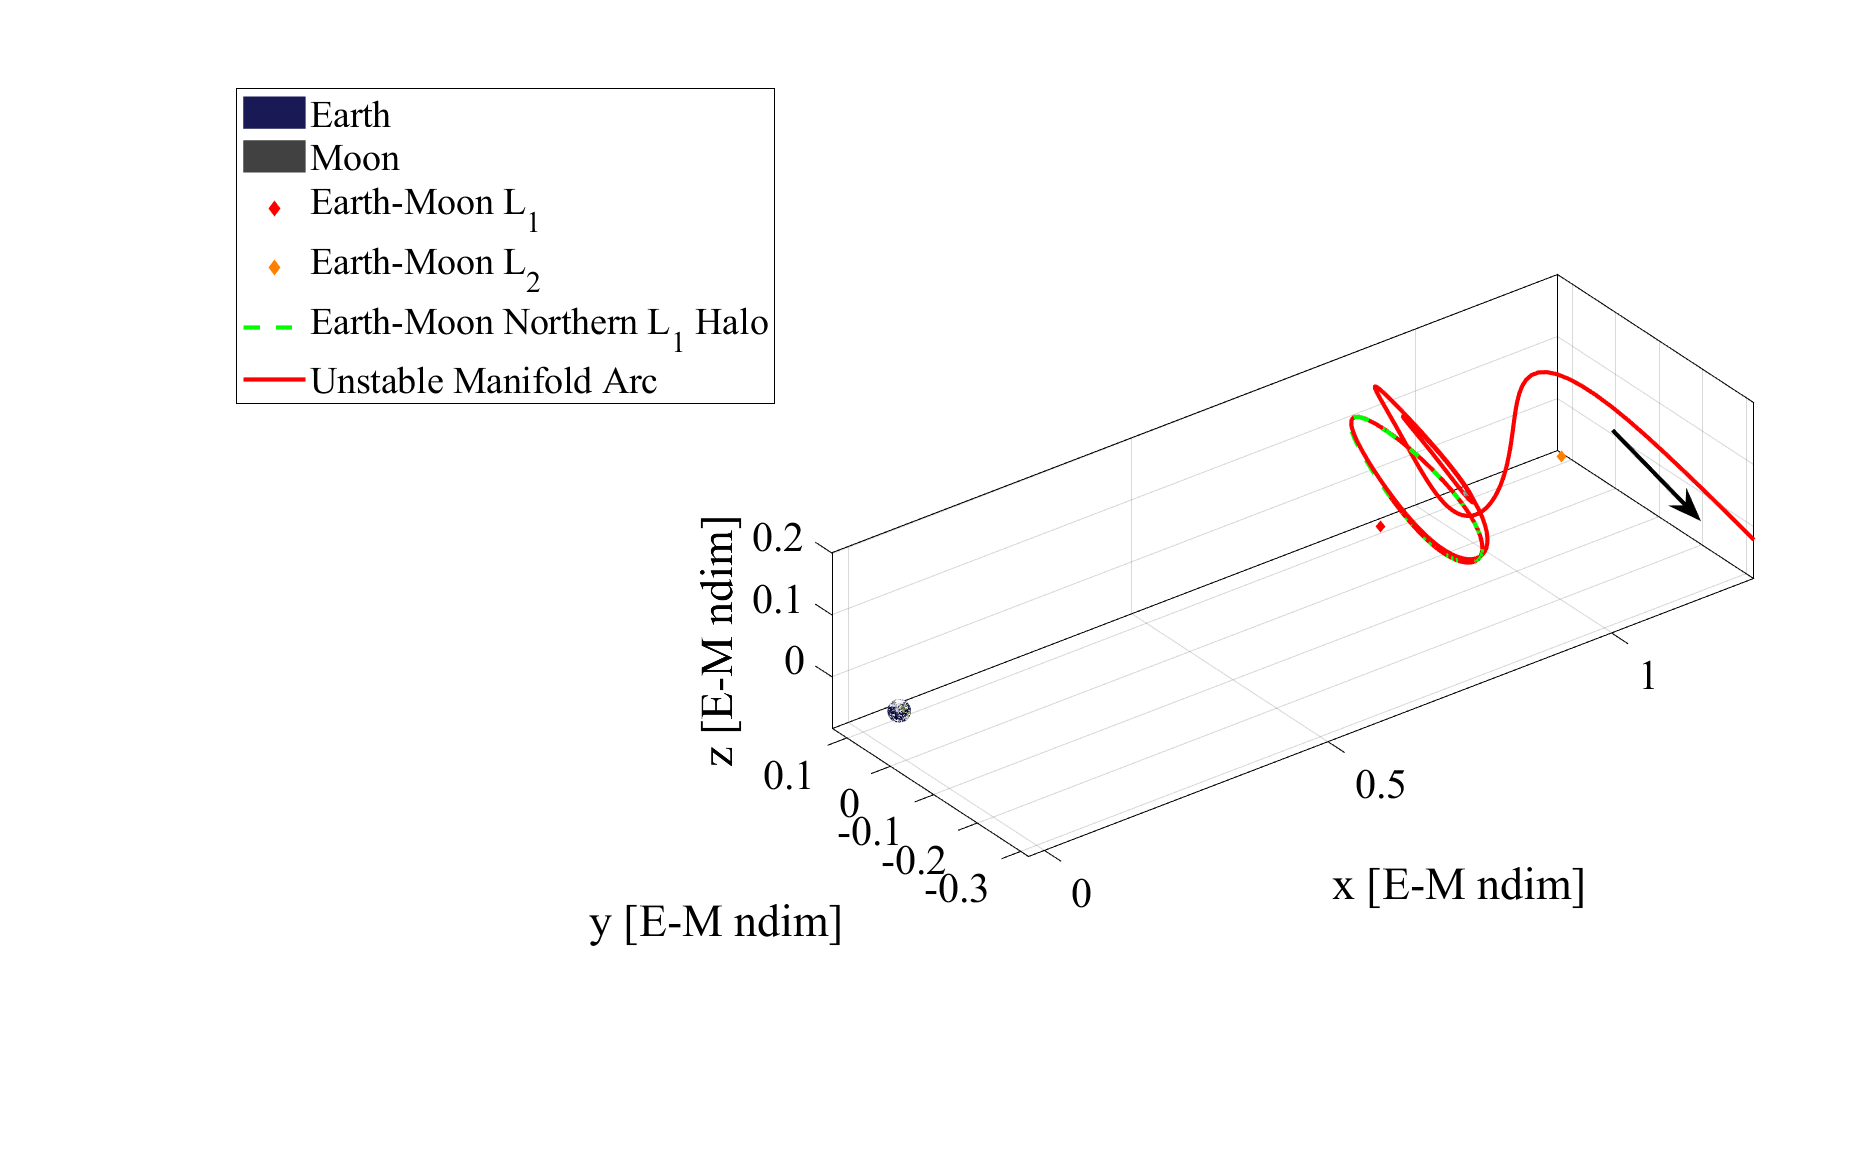
\includegraphics[width=0.9\textwidth]{figures/StagedMinDvEM.pdf}
    \caption{Northern $L_{1}$ halo orbit ($JC=3.03$) departure manifold arc in the Earth-Moon barycentric rotating frame for a low-$\Delta v$ case.}
    \label{fig:stagedMinDvEM}
\end{figure}

\begin{figure}[H]
    \centering
    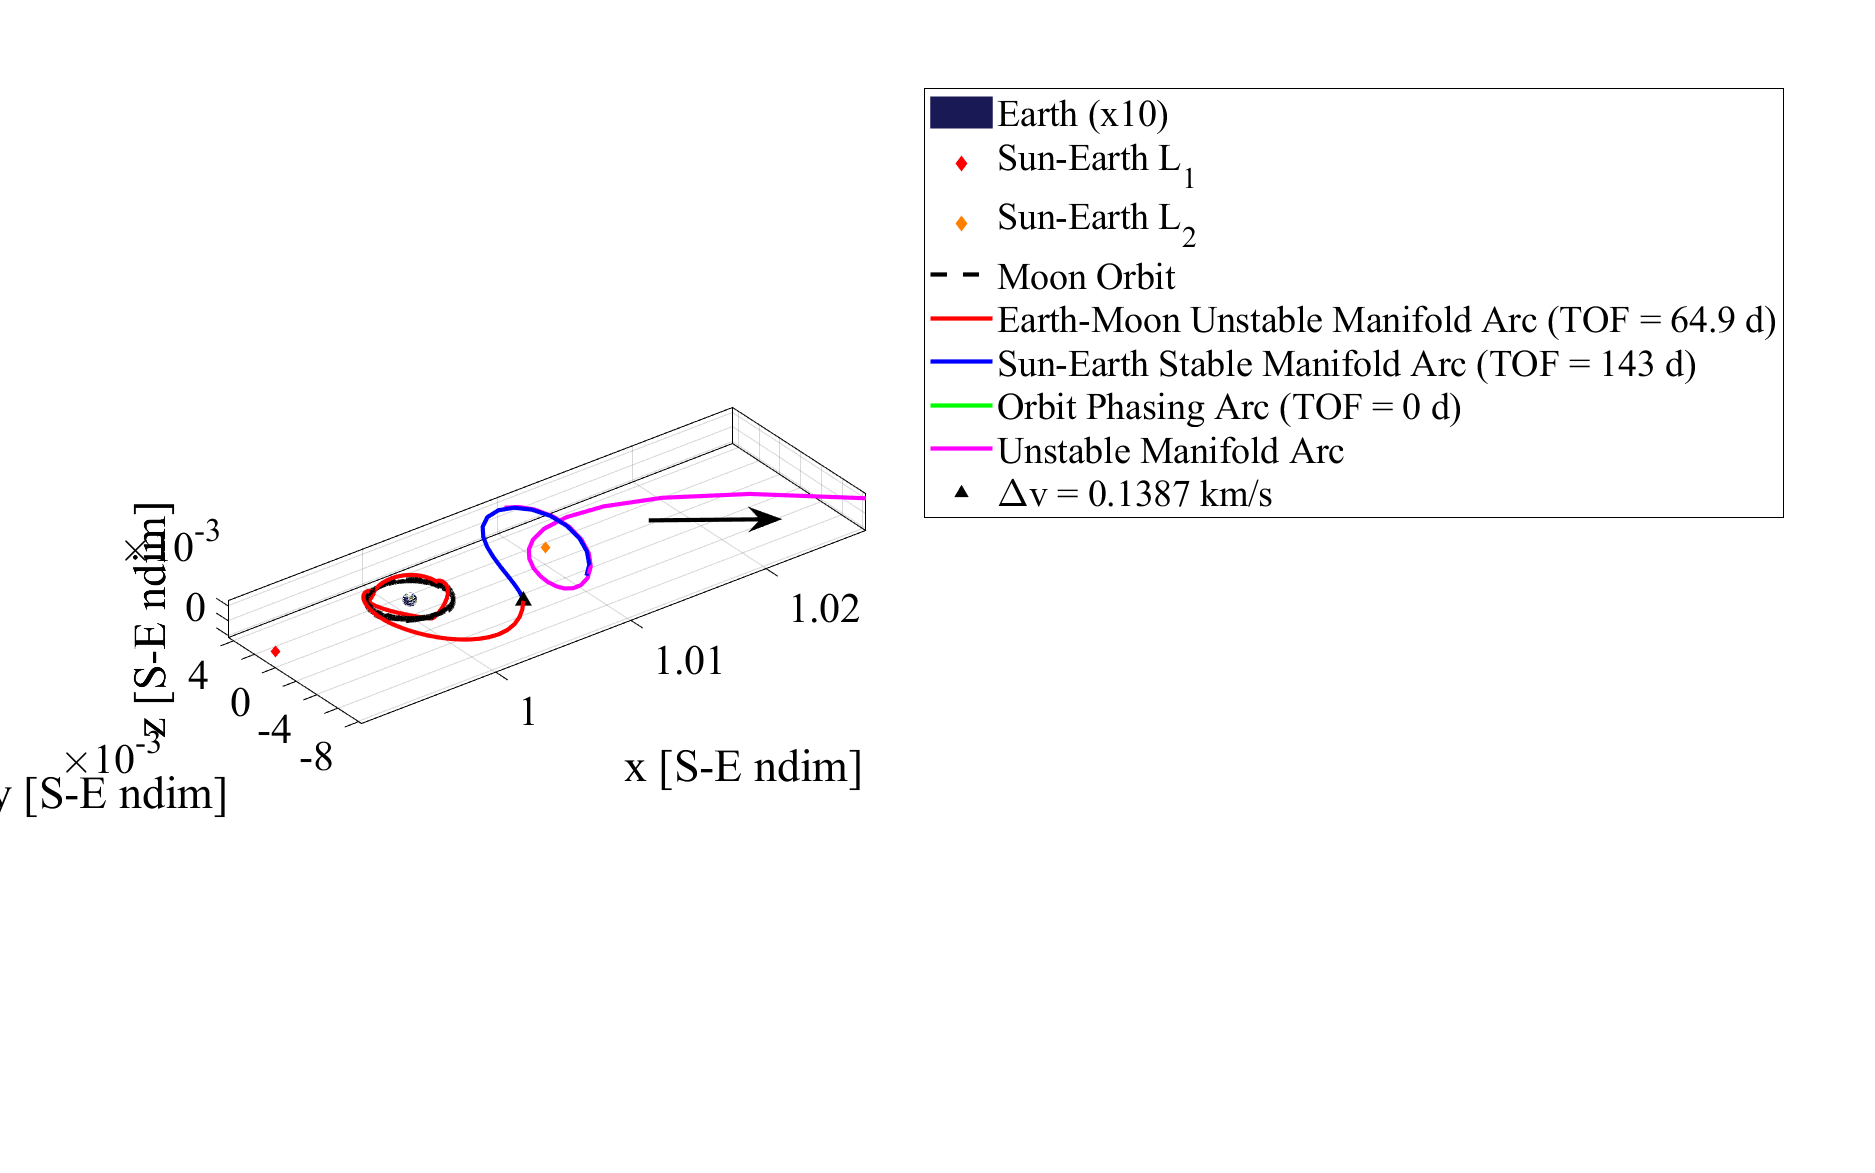
\includegraphics[width=0.9\textwidth]{figures/StagedMinDvSE.pdf}
    \caption{Departure CR3BP arc with northern $L_{2}$ halo staging orbit ($JC=3.000808$) in the Sun-Earth rotating frame for a low-$\Delta v$ case.}
    \label{fig:stagedMinDvSE}
\end{figure}

\begin{figure}[H]
    \centering
    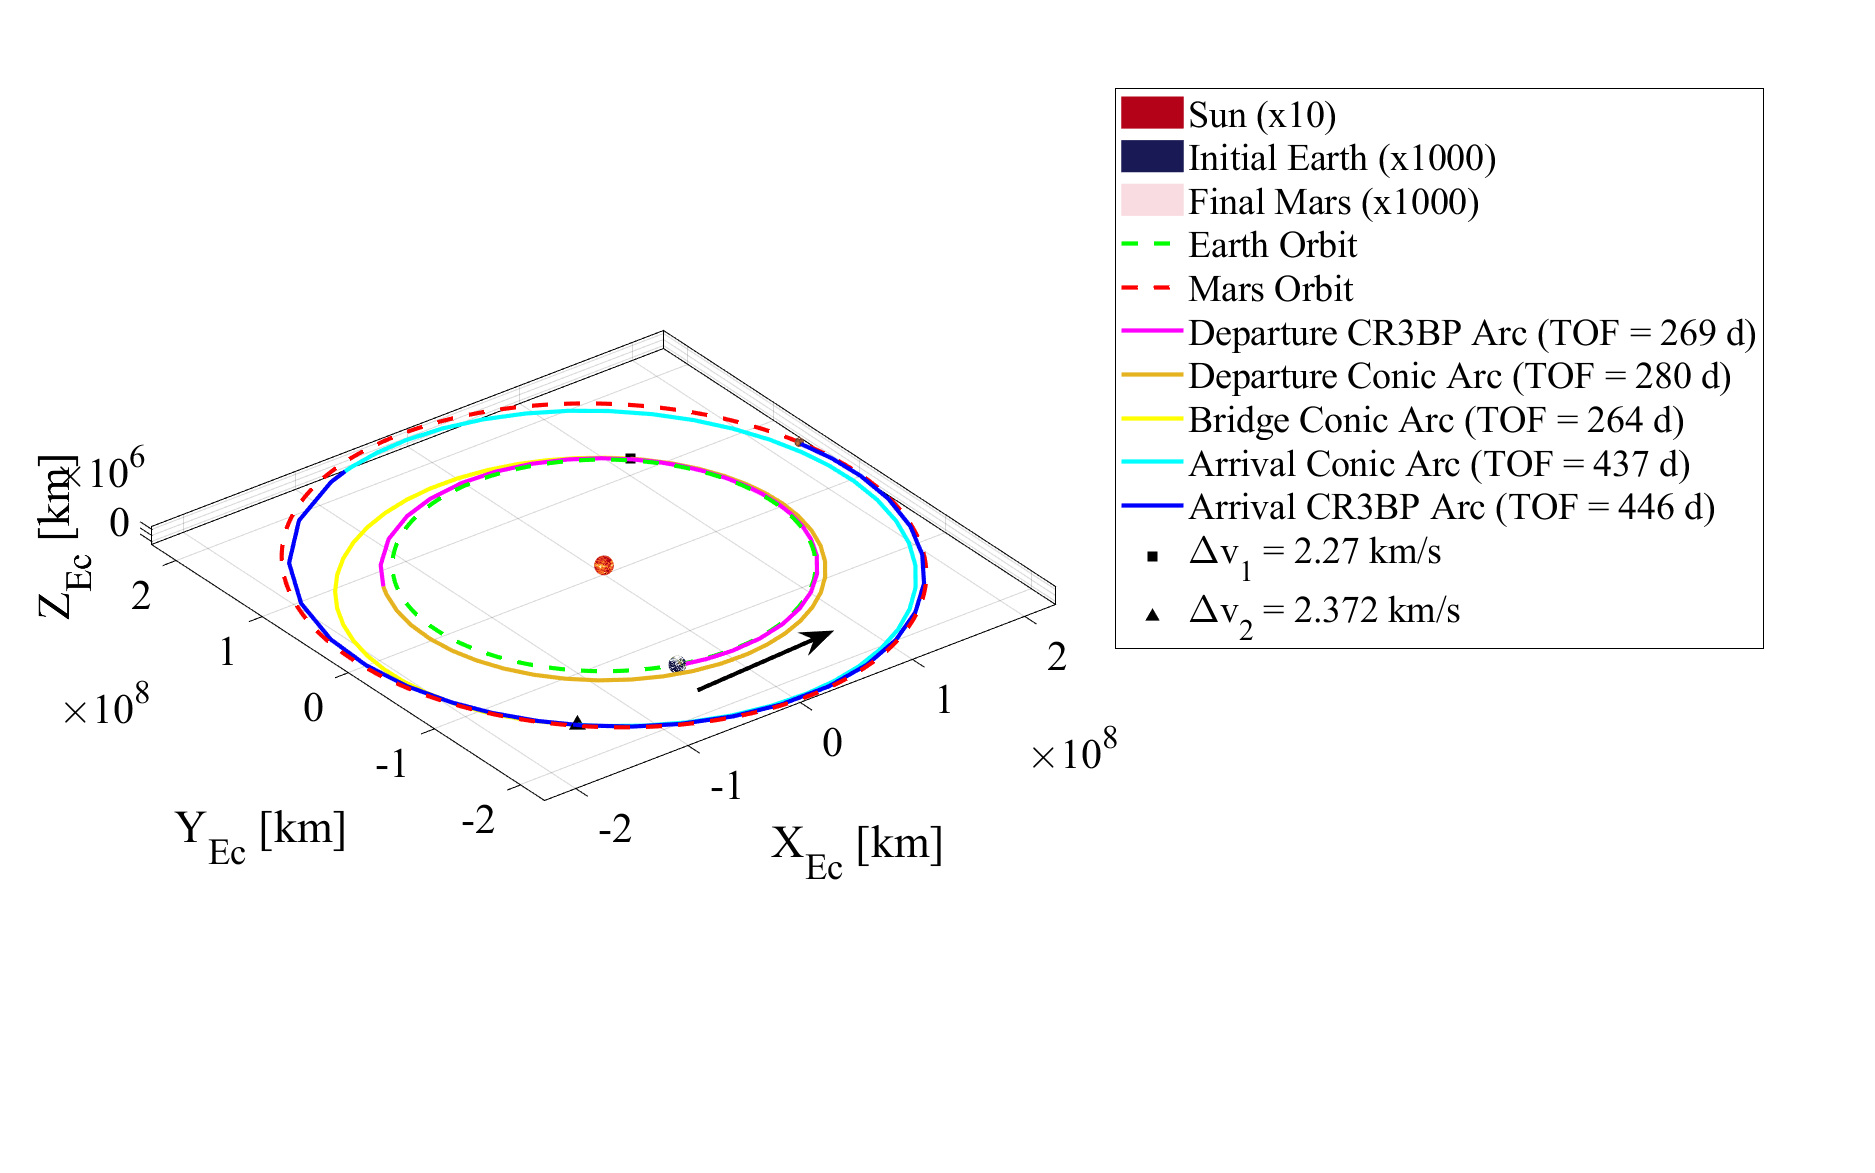
\includegraphics[width=0.9\textwidth]{figures/StagedMinDvMMAT.pdf}
    \caption{MMAT in the Sun-centered Ecliptic J2000 frame for a staging orbit low-$\Delta v$ case.}
    \label{fig:stagedMinDvMMAT}
\end{figure}
\vspace{20mm}

\begin{figure}[H]
    \begin{subfigure}[h]{0.495\linewidth}
        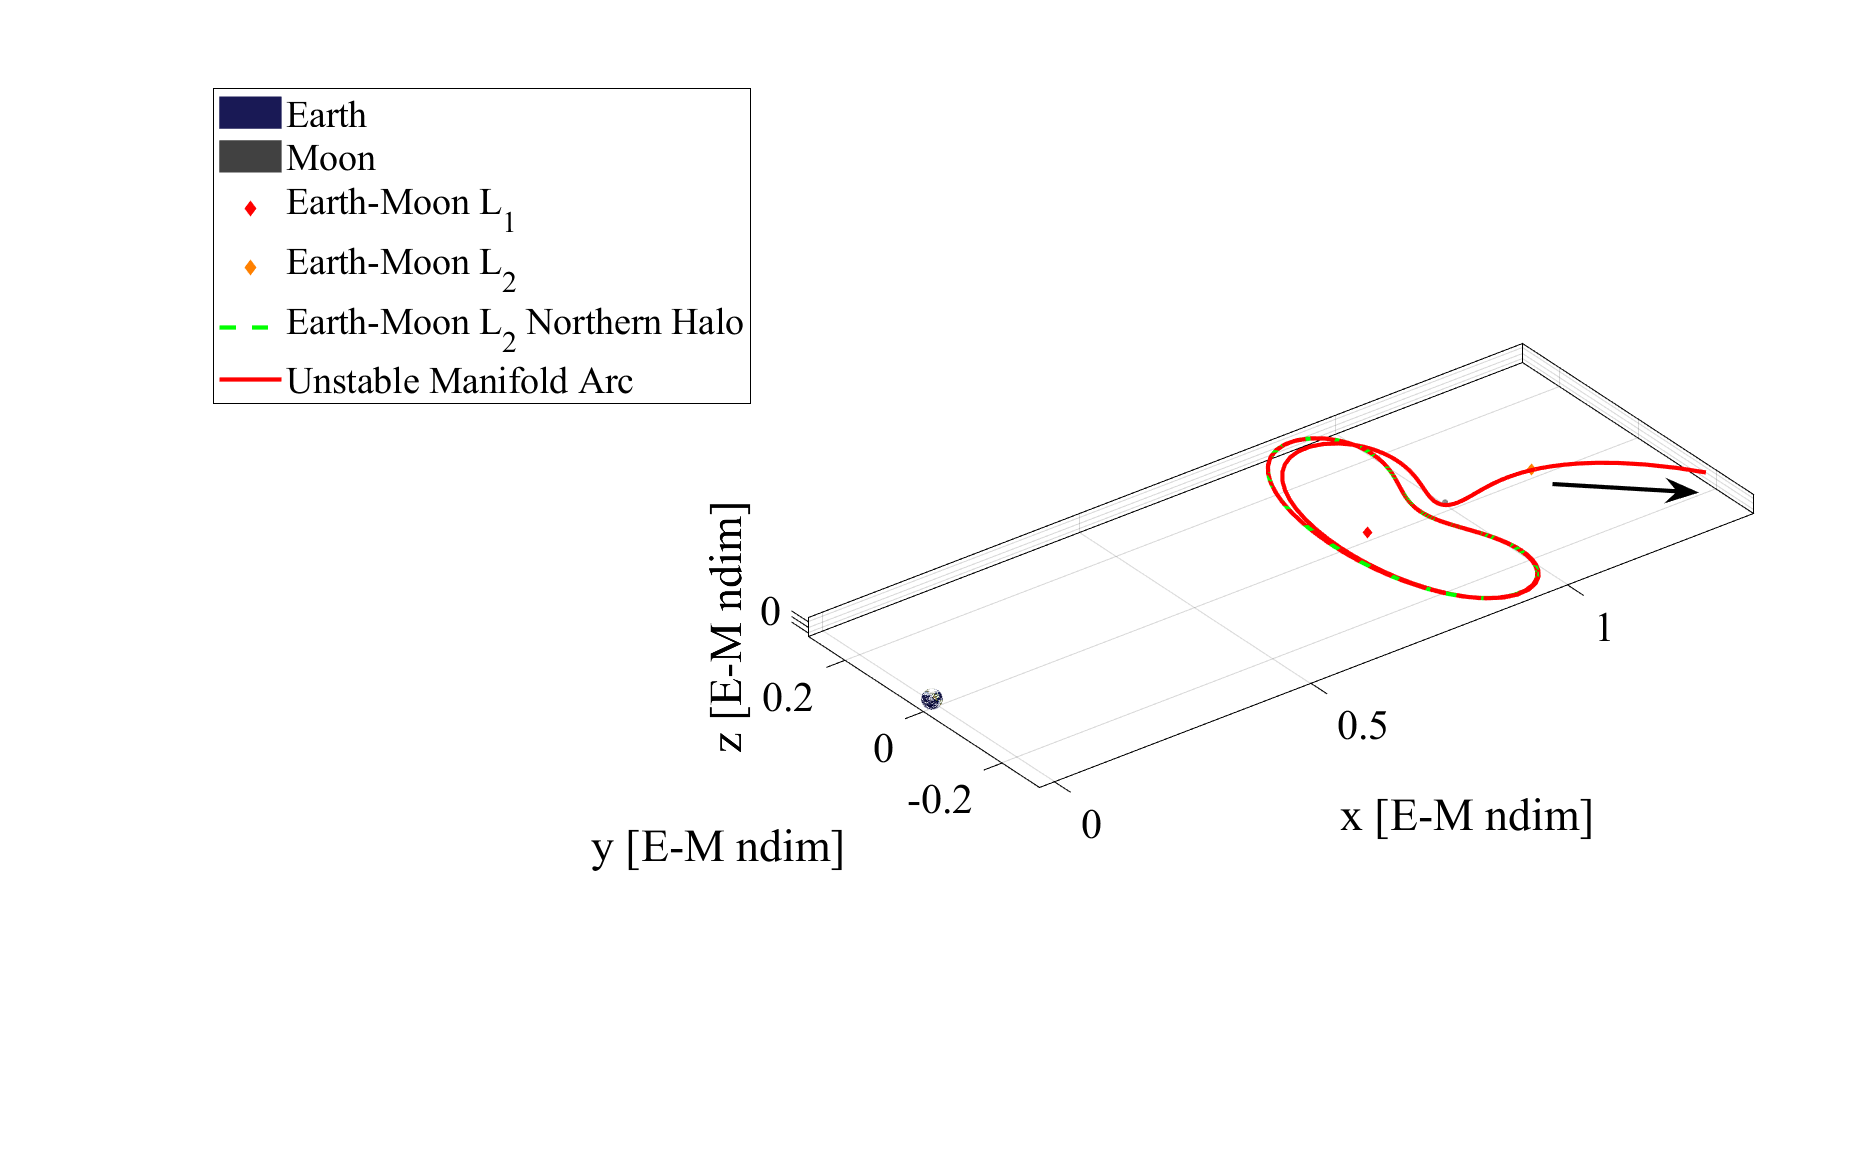
\includegraphics[width=\textwidth]{figures/DirectMinDvEM.pdf}
        \caption{Earth-Moon barycentric rotating frame.}
    \end{subfigure}
    \hfill
    \begin{subfigure}[h]{0.495\linewidth}
        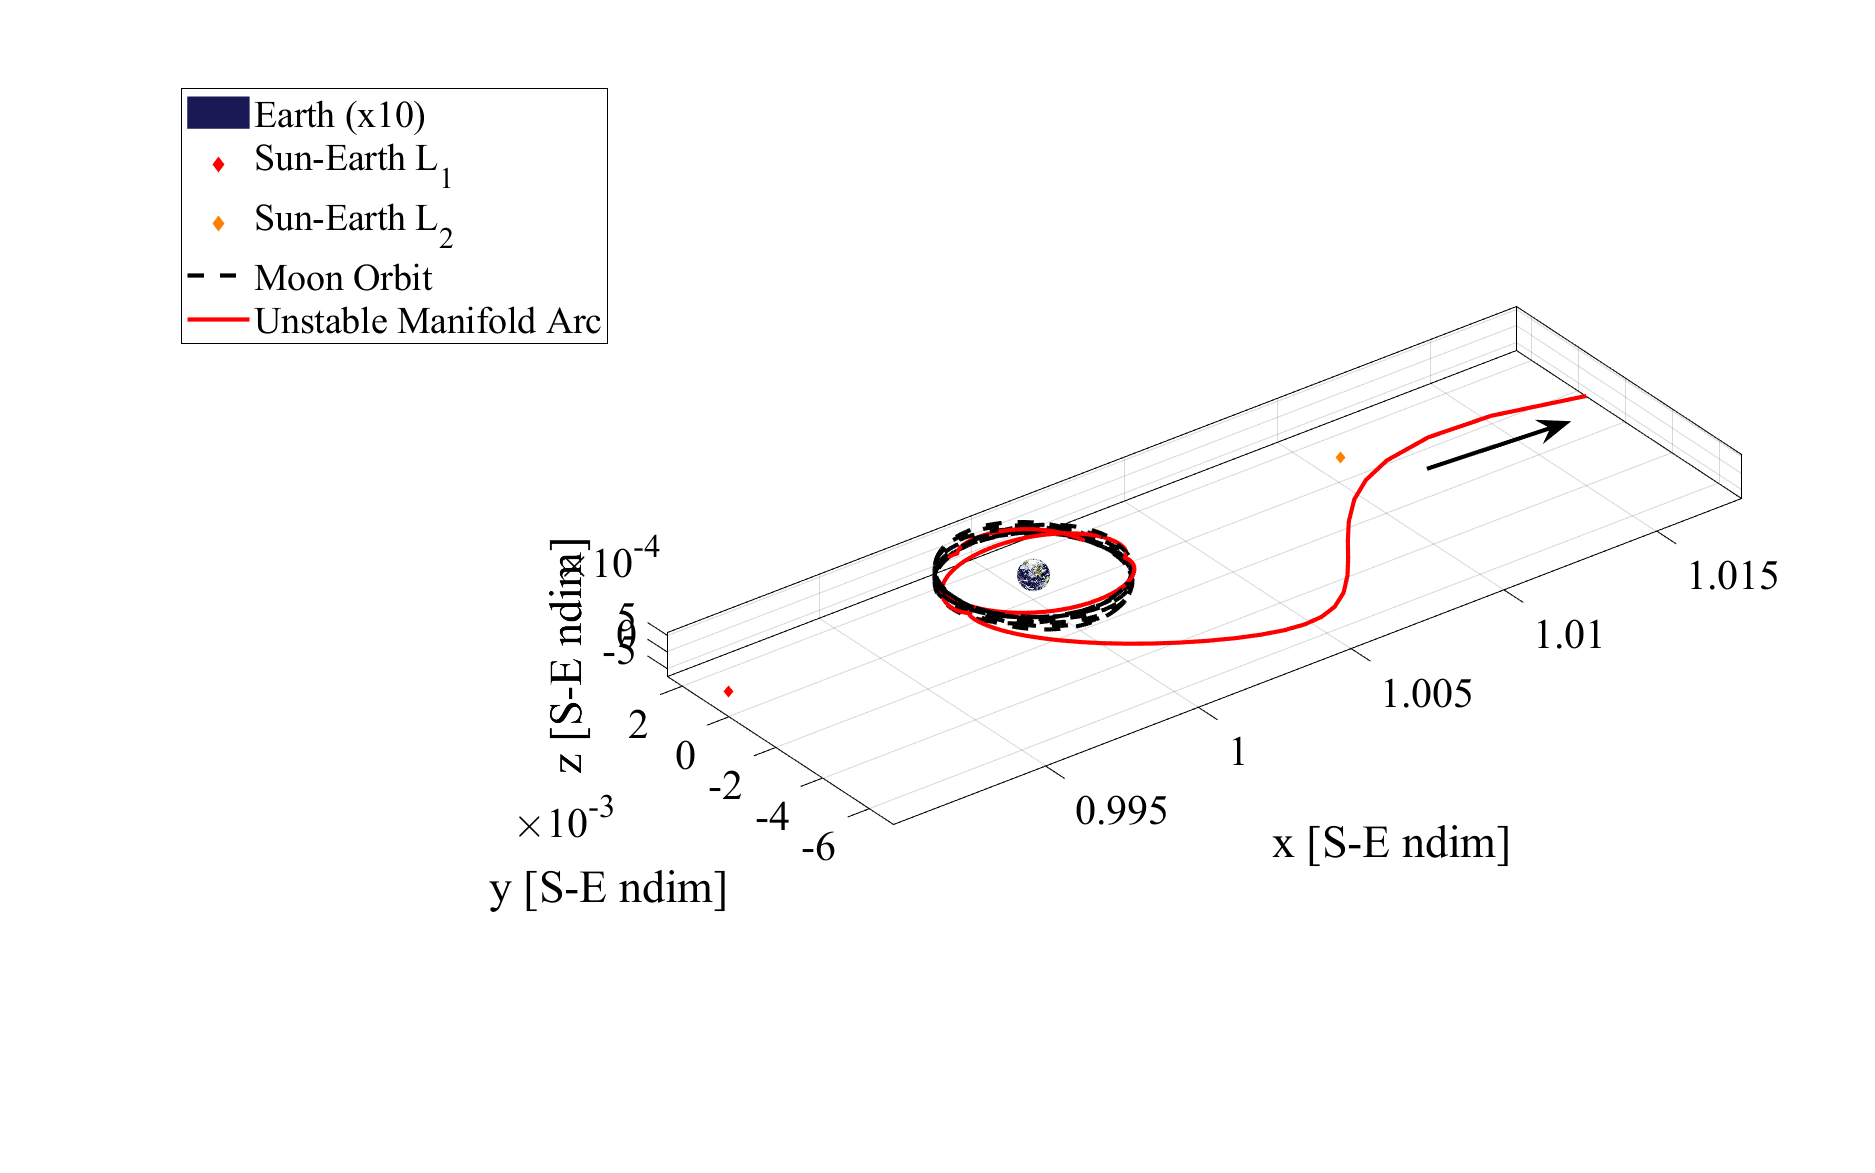
\includegraphics[width=\textwidth]{figures/DirectMinDvSE.pdf}
        \caption{Sun-Earth barycentric rotating frame.}
    \end{subfigure}
    \caption{$L_{1}$ Lyapunov orbit ($JC=3.0$) departure CR3BP arc for a low-$\Delta v$ case.}
    \label{fig:directMinDvE}
\end{figure}

\begin{figure}[H]
    \centering
    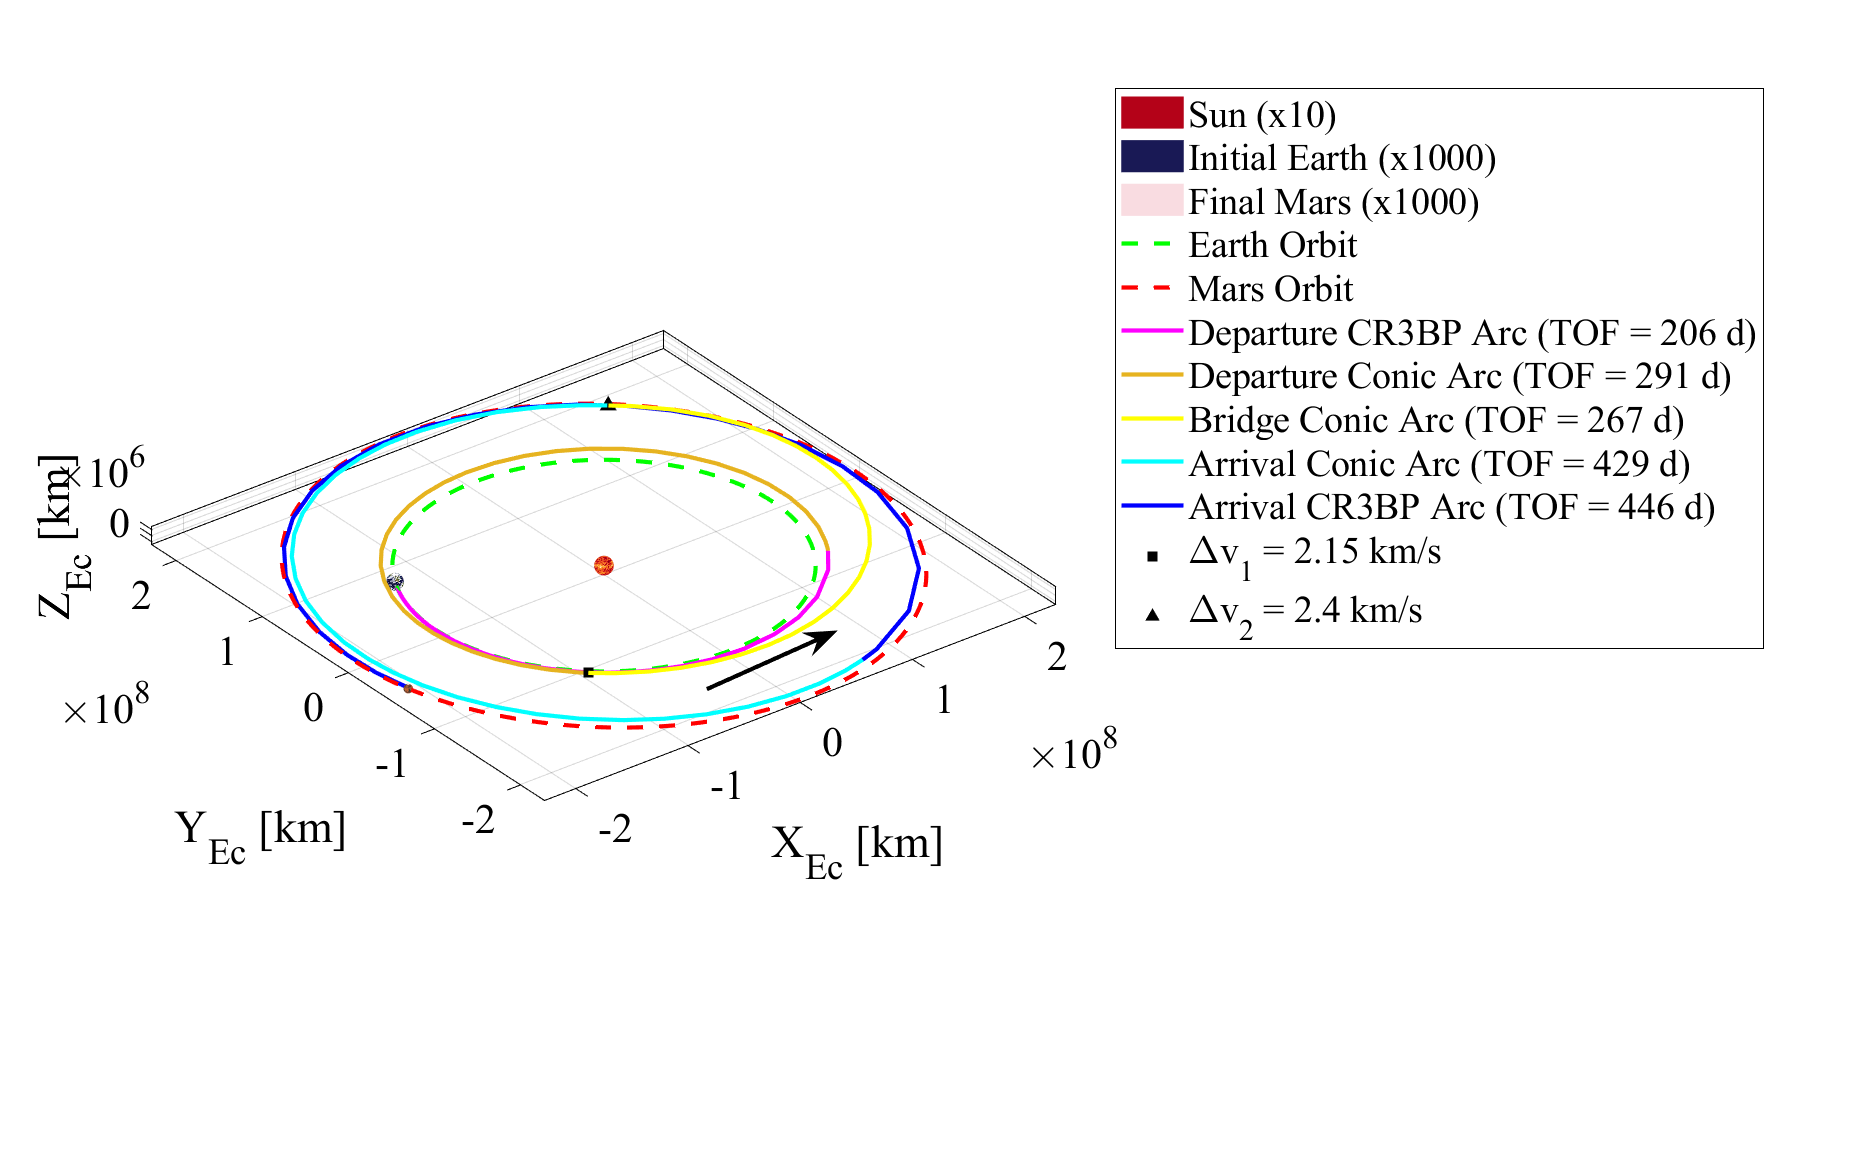
\includegraphics[width=0.9\textwidth]{figures/DirectMinDvMMAT.pdf}
    \caption{MMAT in the Sun-centered Ecliptic J2000 frame for a direct low-$\Delta v$ case.}
    \label{fig:directMinDvMMAT}
\end{figure}

Beyond the relative orientation between the two MMAT maneuvers, the energy gap between the
departure and arrival arcs (and thereby the Sun-Earth and Sun-Mars CR3BP manifold arcs,
respectively) also contributes to the total $\Delta v$. A larger difference requires a higher
magnitude maneuver to change the Keplerian conic energy from the departure arc to that of the
arrival arc, which are determined by the manifold arcs selected and the phasing of the two
planetary systems, highlighting the importance of families of transfer solutions. Since several
interdependent factors affect the total maneuver cost, it is necessary to search through the
results across families of solutions to find low-$\Delta v$ solution basins.

\subsection{Contributing Factors for Lower Total Times-of-Flight}
While maneuver cost is primarily dependent on the final MMAT maneuver location, the biggest factor
affecting time-of-flight is the relative orientation of the departure and arrival conic arcs. Since
the orientations are dependent on their respective CR3BP manifold arcs, the phasing of the two
planetary systems at departure and arrival largely dictate the total transfer TOF. As mentioned,
the first MMAT maneuver occurs at the periapsis of the departure conic arc. Consequently, to
minimize the time along the departure conic arc, its periapsis should be just after the Sun-Earth
CR3BP SoI intersection. Similarly, although the true anomaly of the intersection between the bridge
and arrival arcs varies, it should be just before the Sun-Mars CR3BP SoI intersection true anomaly
to minimize the arrival conic arc TOF. Optimizing the relative timing of the intersections achieves
the shortest possible TOF for the transfer.

The time along the arrival conic arc appears to be easier to decrease than the departure conic arc
TOF. \cref{fig:stagedMinTOFEM}-\cref{fig:stagedMinTOFMMAT} illustrate a low-TOF case from the
lowest-cost staging orbit transfers of a northern $L_{2}$ halo orbit, with a total maneuver cost of
$5.582$ km/s and TOF of $4.25$ years. Departing from the $JC=3.13$ northern $L_{1}$ halo orbit, the
transfer appearing in \cref{fig:directMinTOFE} and \cref{fig:directMinTOFMMAT} has a total maneuver
cost of $5.624$ km/s and TOF of $3.19$ years. In \cref{fig:stagedMinTOFMMAT} and
\cref{fig:directMinTOFMMAT}, the TOF of the arrival conic arc is minimal compared to the other
transfer legs. In the Sun-Earth rotating frame representation, \cref{fig:directMinTOFE}(b), the
manifold arc again departs on the $L_{2}$ side of the Sun-Earth system because the lowest-cost
solutions selected with the cost function tend to be closer to the minimum-$\Delta v$ cases. So the
lowest-TOF transfer among the lowest-cost solutions is still closer to a minimum-$\Delta v$ case.
For the truly minimum-TOF transfers, with maneuver costs much higher than the modified Hohmann
transfer baseline, the unstable manifold arcs depart on the Sun-Earth $L_{1}$ side. The behavior is
consistent for lower-TOF direct transfers across all the departure orbits analyzed in this
investigation.

A few other ways to reduce the total transfer TOF involve the other three legs of the transfer.
Although the minimum-$\Delta v$ transfers occur when the bridge and arrival conic arc intersection
is $\ang{180}$ from the first MMAT maneuver, the bridge arc TOF is decreased by moving the final
maneuver closer to the periapsis. While the maneuver cost increases, it is sometimes worth the TOF
savings. Another option is to decrease the departure and arrival CR3BP manifolod arc
times-of-flight by changing the invariant manifold arc selection. Some manifold arcs depart
the system faster than others from the same orbit and can lead to slight decreases in TOF. The
proposed adjustments demonstrate the flexibility in optimizing transfer trajectories by balancing
maneuver costs with time-of-flight reductions across individual segments of the transfer.

\begin{figure}[H]
    \centering
    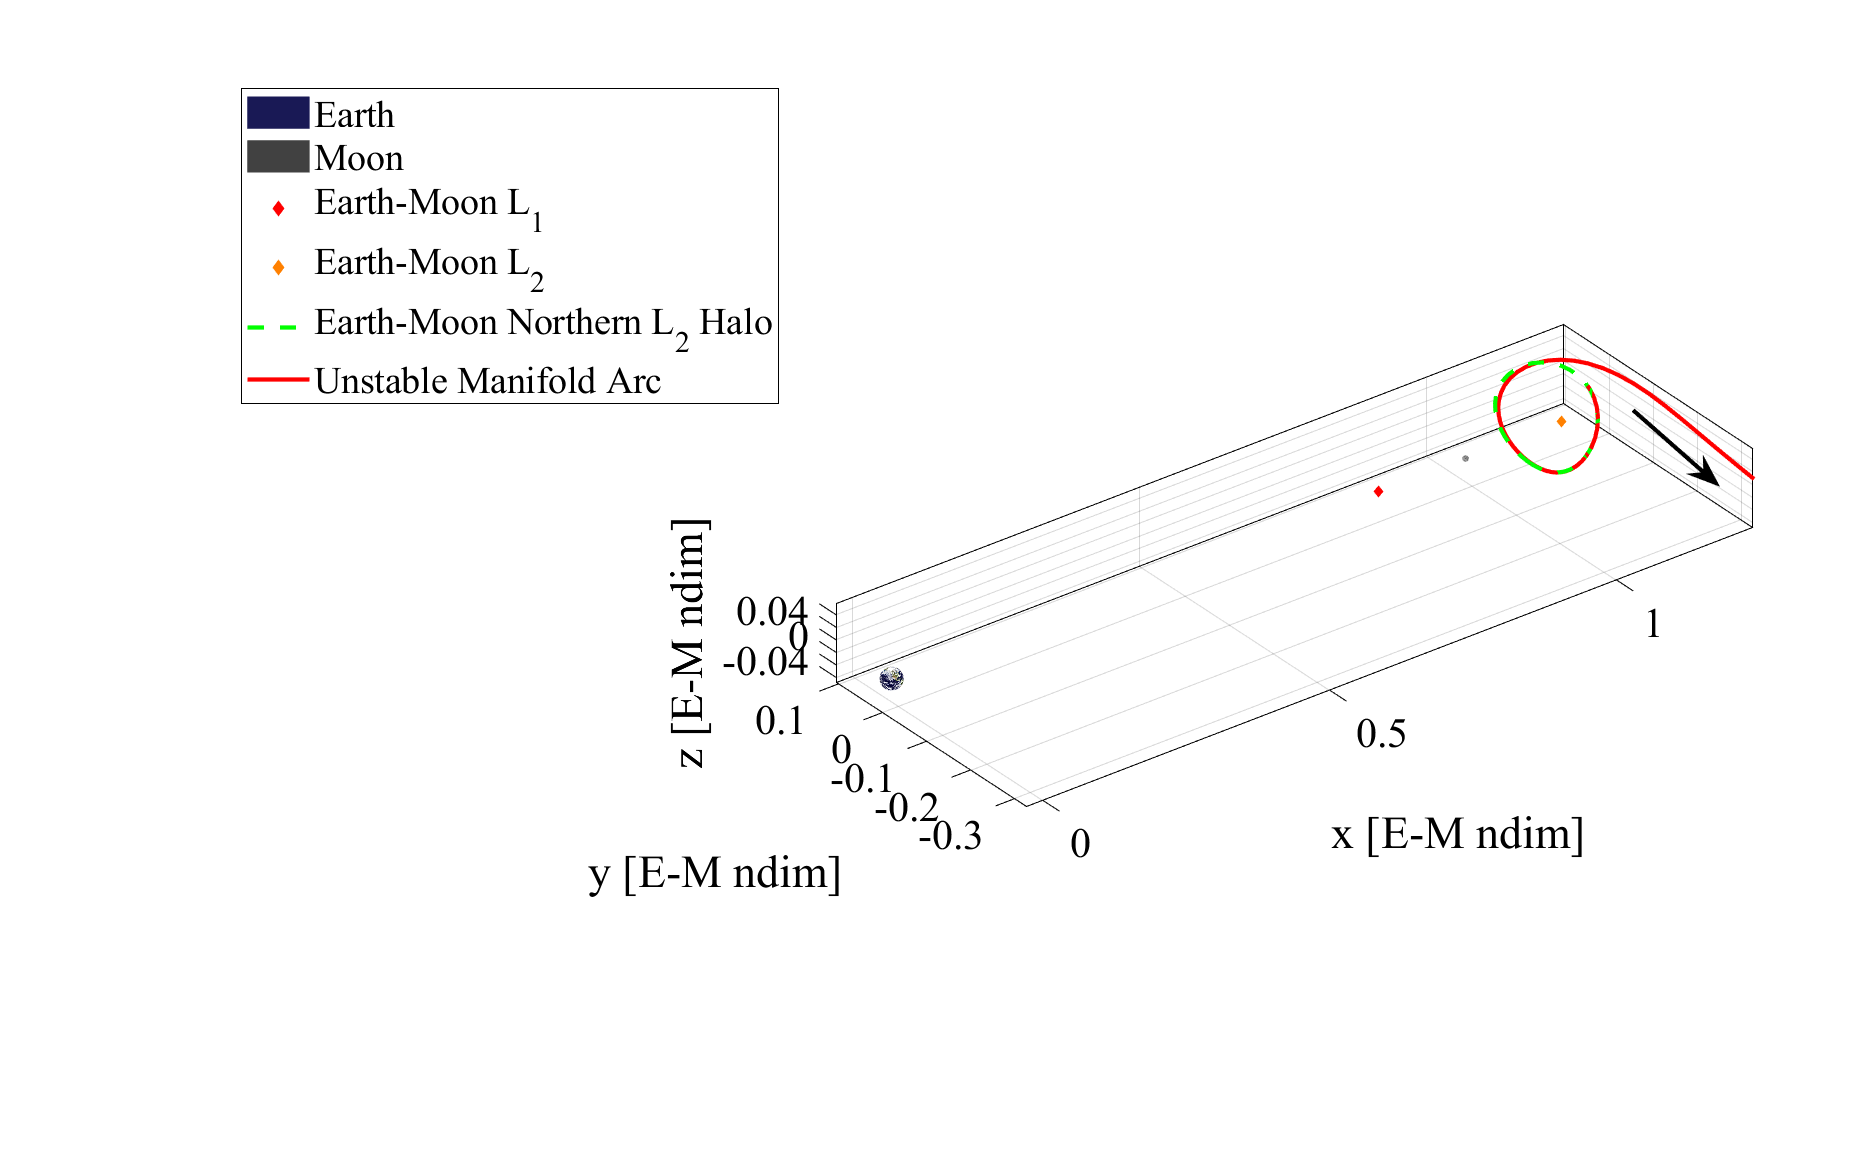
\includegraphics[width=0.9\textwidth]{figures/StagedMinTOFEM.pdf}
    \caption{Northern $L_{2}$ halo orbit ($JC=3.13$) departure manifold arc in the Earth-Moon barycentric rotating frame for a low-TOF case.}
    \label{fig:stagedMinTOFEM}
\end{figure}

\begin{figure}[H]
    \centering
    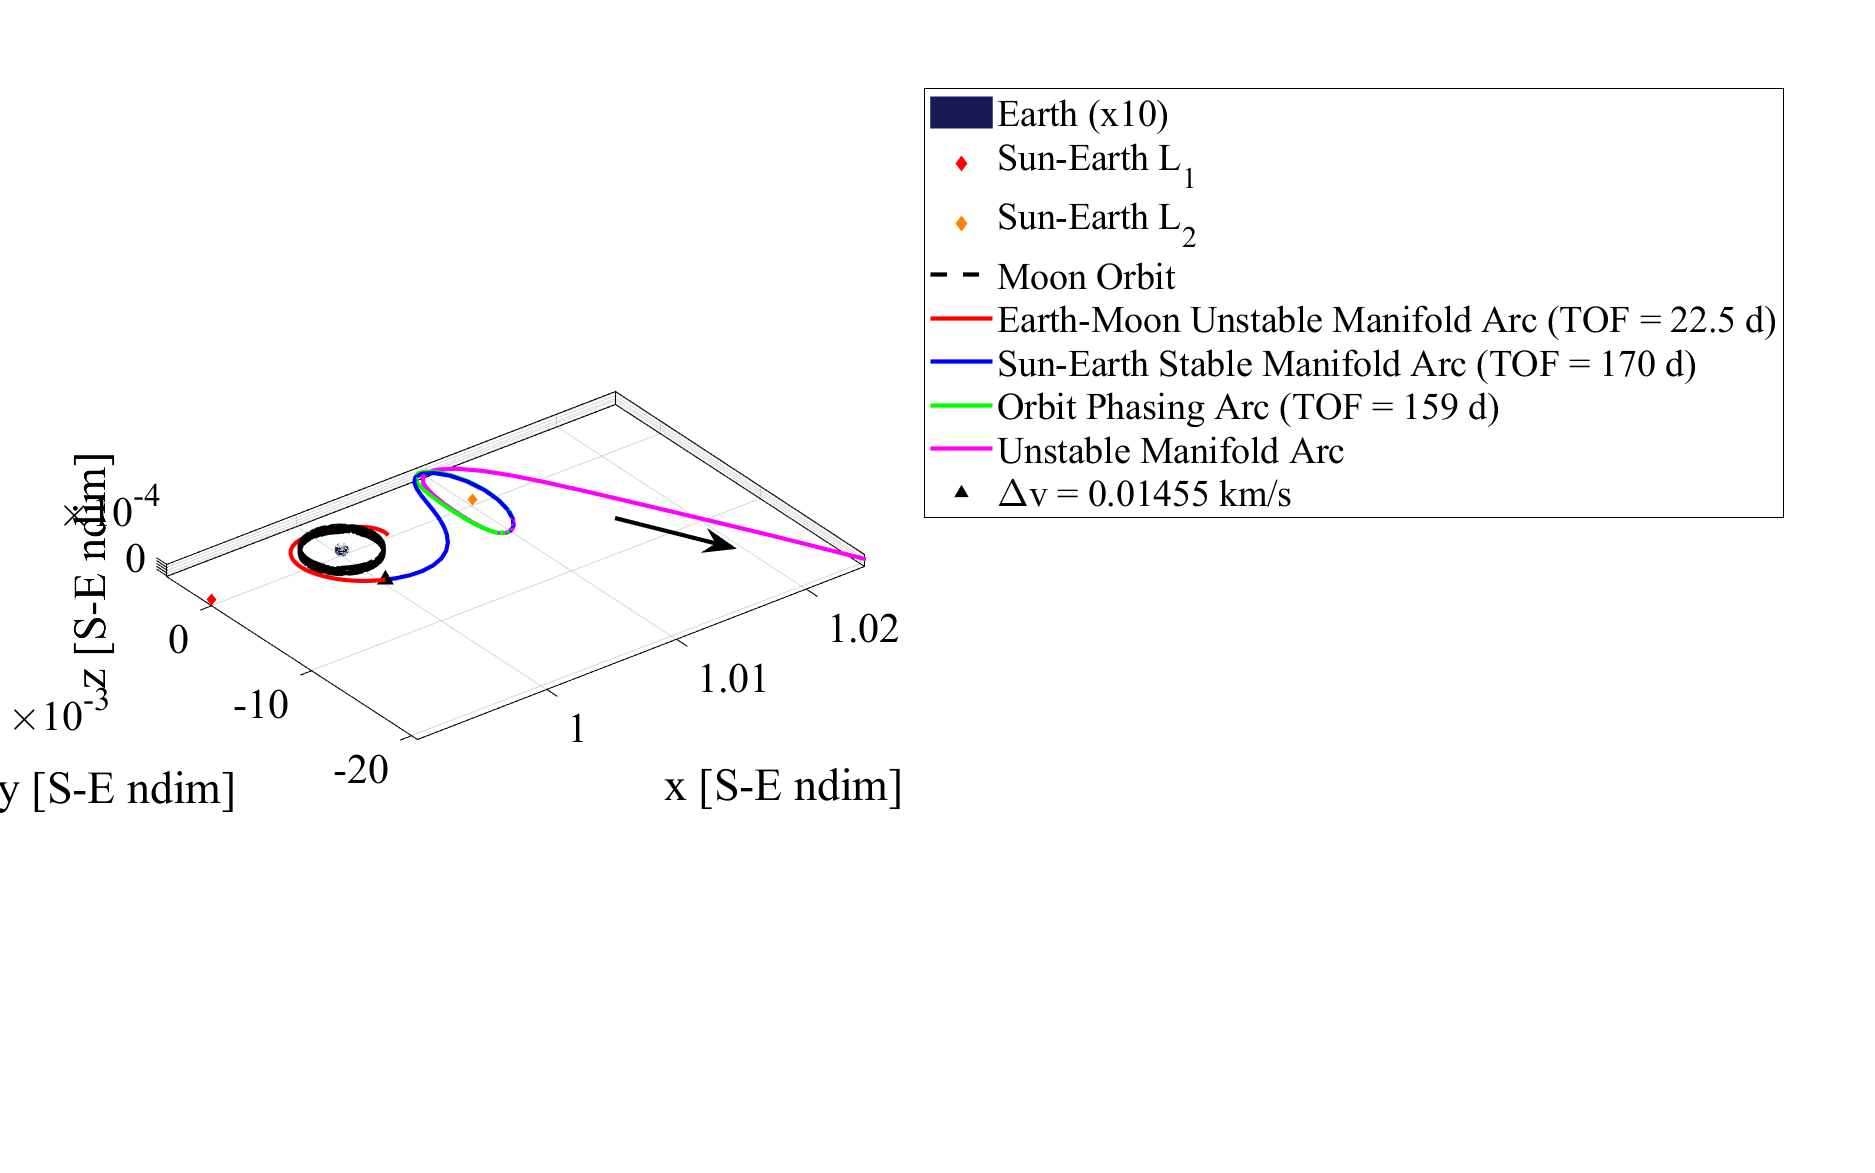
\includegraphics[width=0.9\textwidth]{figures/StagedMinTOFSE.pdf}
    \caption{Departure CR3BP arc with northern $L_{2}$ halo staging orbit ($JC=3.0008189$) in the Sun-Earth rotating frame for a low-TOF case.}
    \label{fig:stagedMinTOFSE}
\end{figure}

\begin{figure}[H]
    \centering
    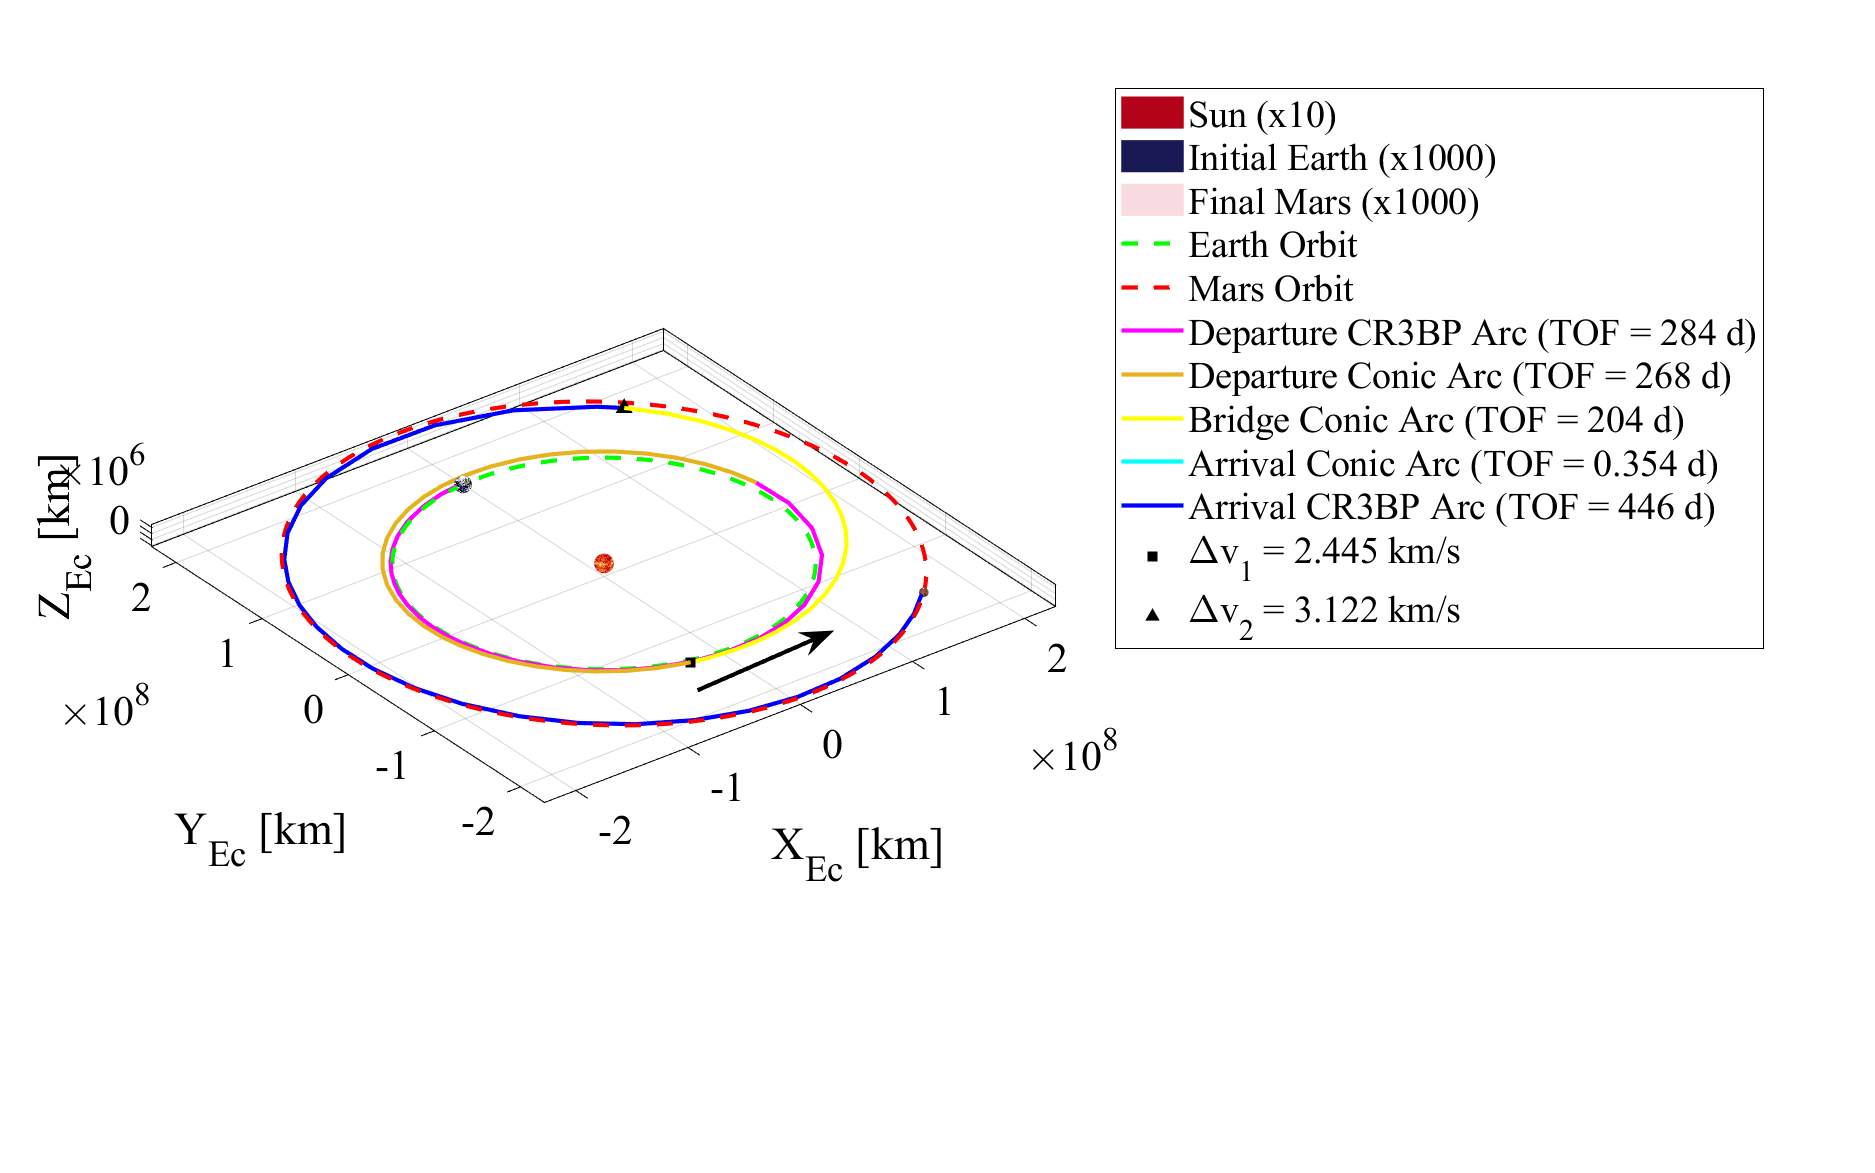
\includegraphics[width=0.9\textwidth]{figures/StagedMinTOFMMAT.pdf}
    \caption{MMAT in the Sun-centered Ecliptic J2000 frame for a staging orbit low-TOF case.}
    \label{fig:stagedMinTOFMMAT}
\end{figure}

\begin{figure}[H]
    \begin{subfigure}[h]{0.495\linewidth}
        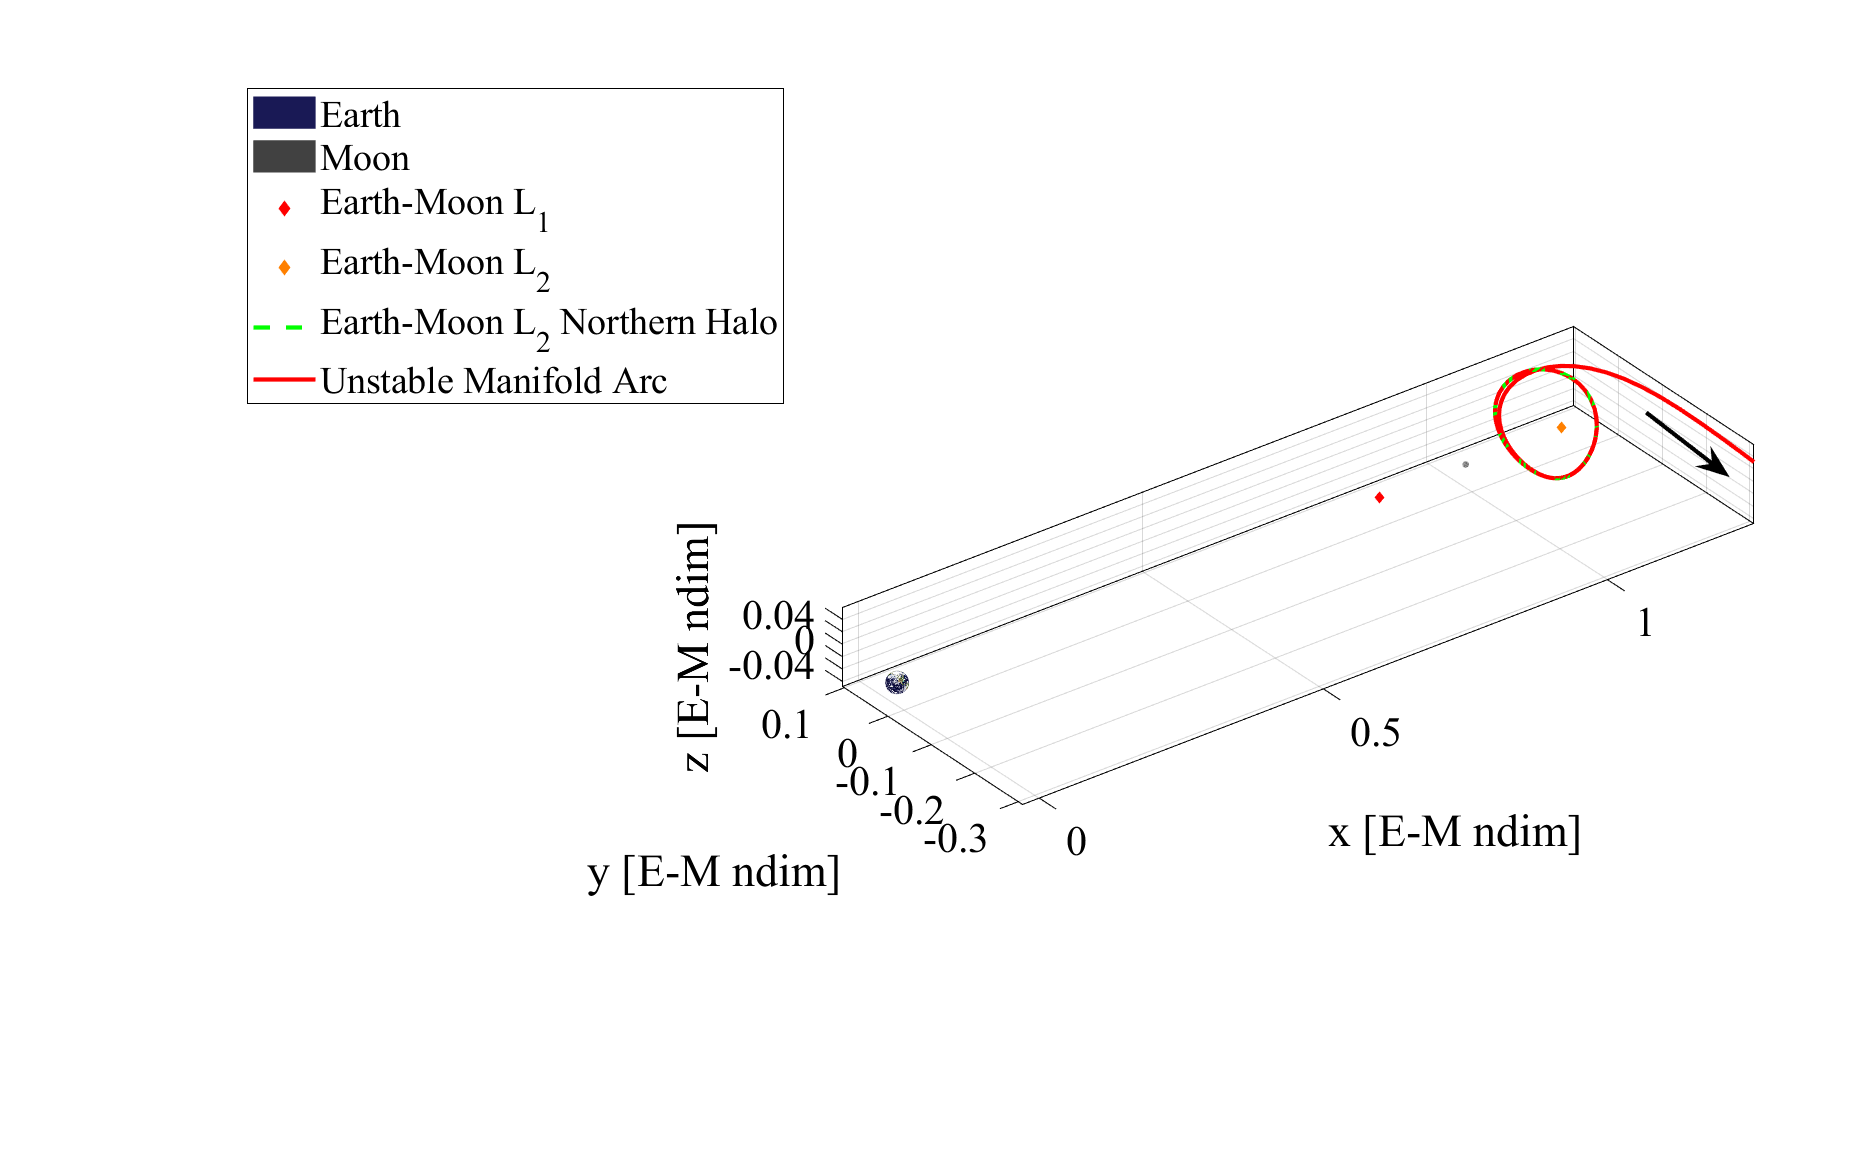
\includegraphics[width=\textwidth]{figures/DirectMinTOFEM.pdf}
        \caption{Earth-Moon barycentric rotating frame.}
    \end{subfigure}
    \hfill
    \begin{subfigure}[h]{0.495\linewidth}
        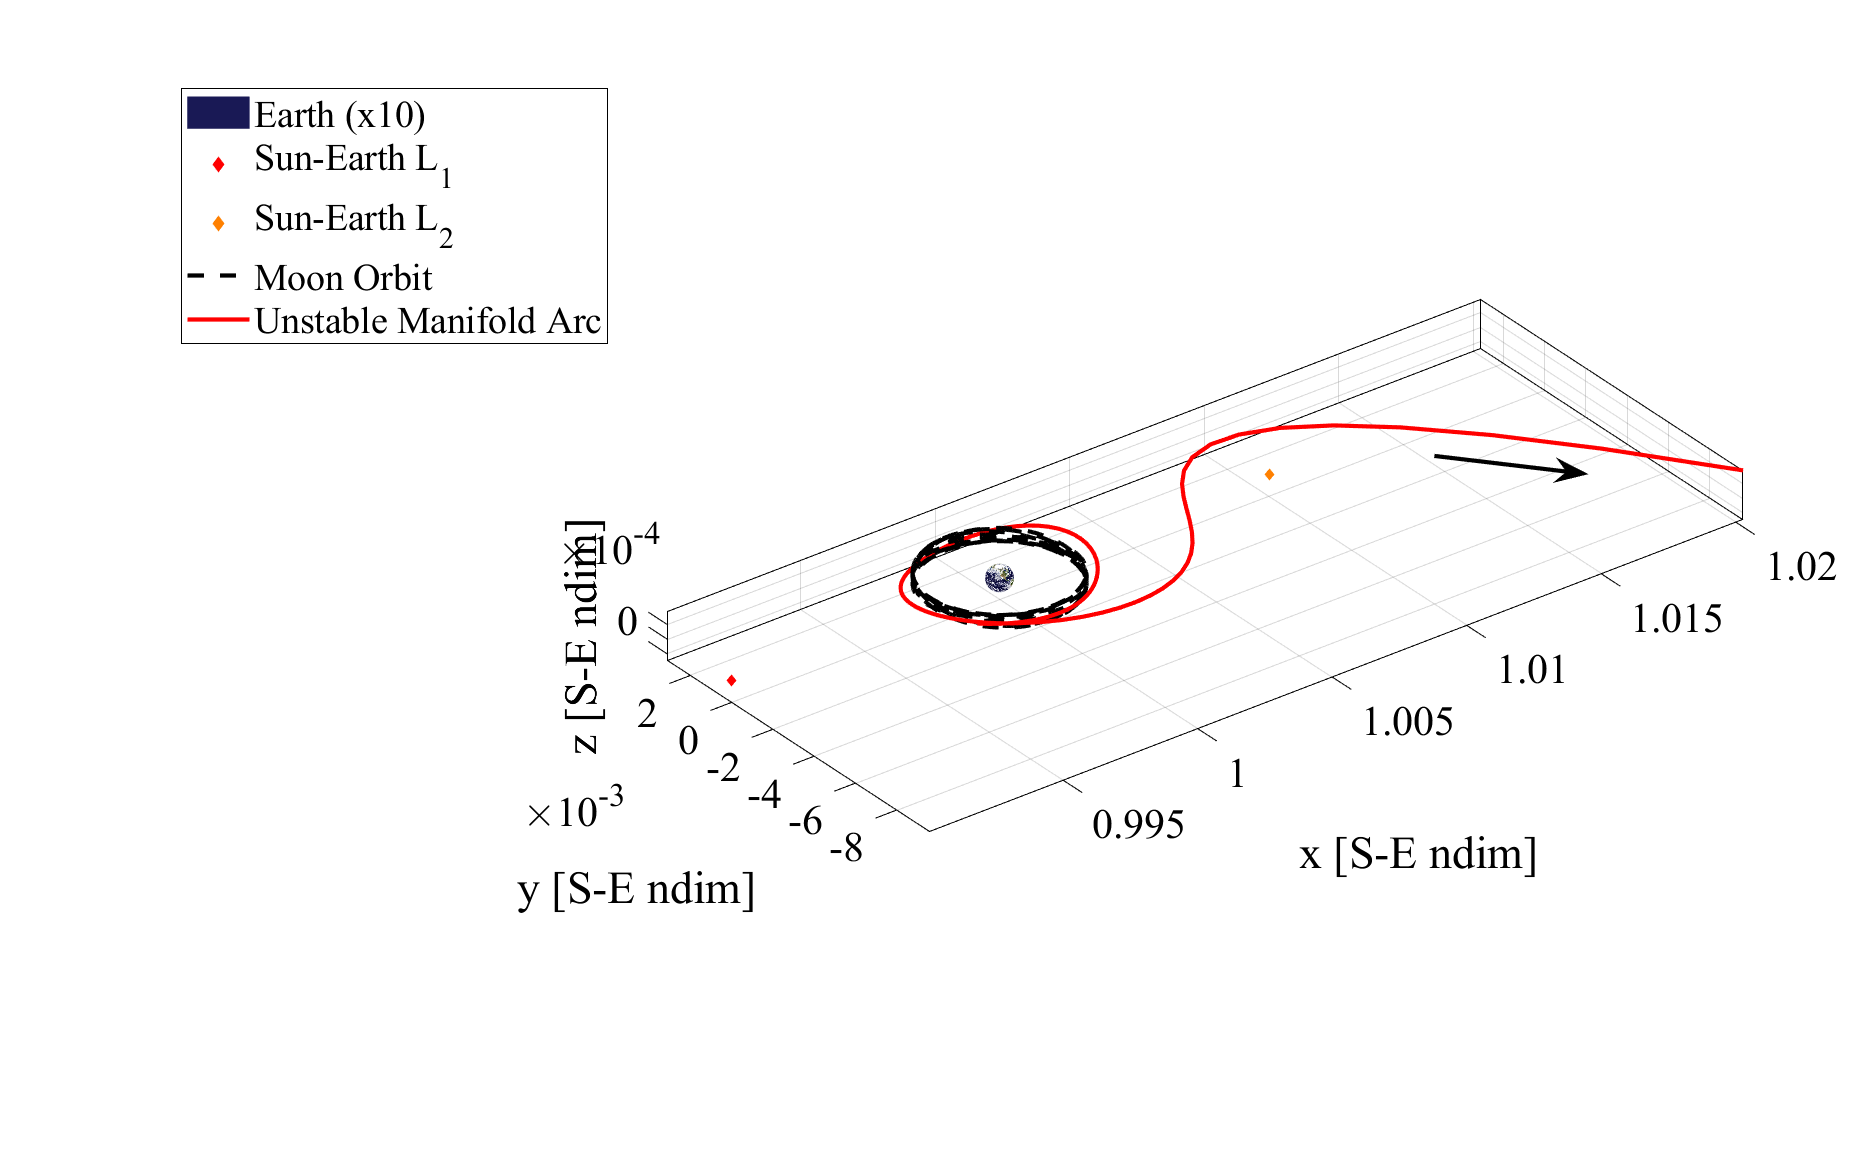
\includegraphics[width=\textwidth]{figures/DirectMinTOFSE.pdf}
        \caption{Sun-Earth barycentric rotating frame.}
    \end{subfigure}
    \caption{Northern $L_{2}$ halo orbit ($JC=3.13$) departure CR3BP arc for a low-TOF case.}
    \label{fig:directMinTOFE}
\end{figure}

\begin{figure}[H]
    \centering
    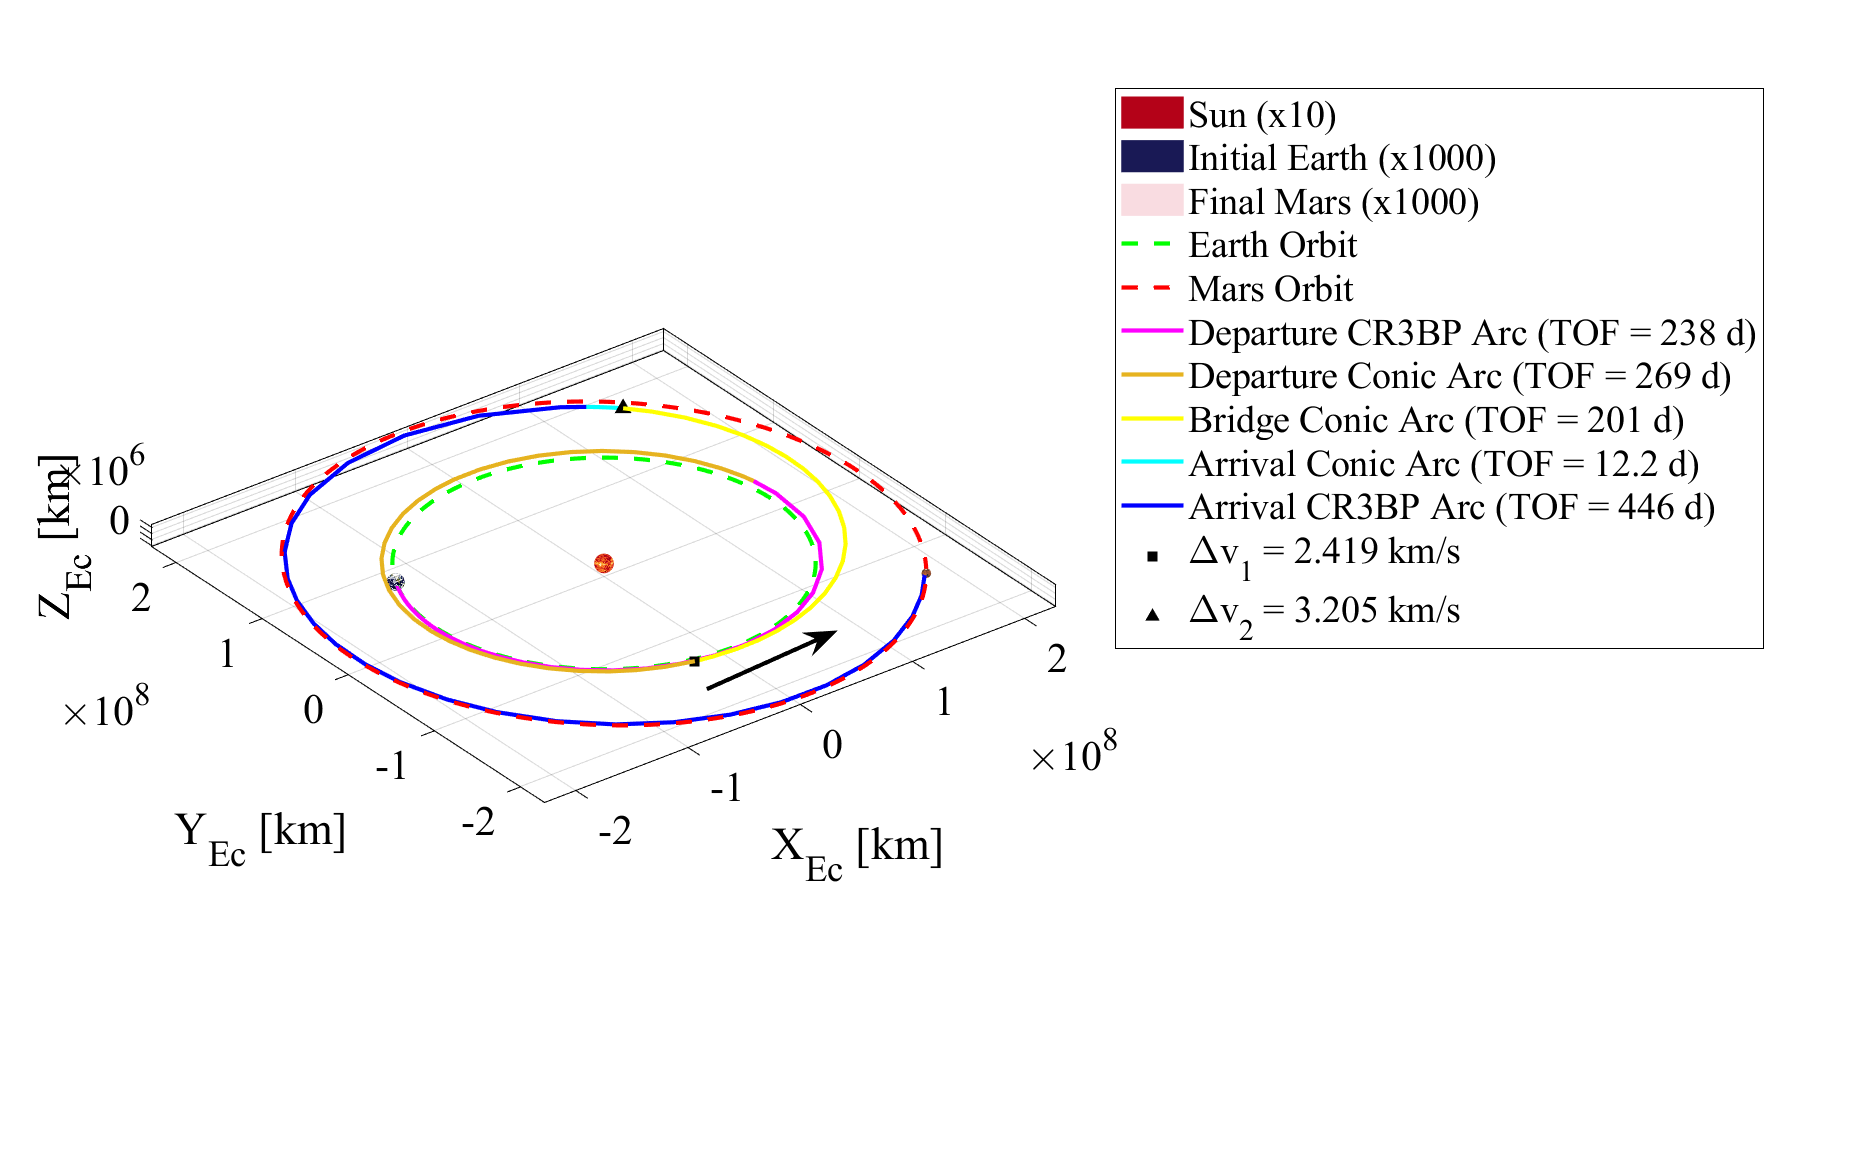
\includegraphics[width=0.9\textwidth]{figures/DirectMinTOFMMAT.pdf}
    \caption{MMAT in the Sun-centered Ecliptic J2000 frame for a direct low-TOF case.}
    \label{fig:directMinTOFMMAT}
\end{figure}

\subsection{Comparison between Departure Orbits}
Since both categories of transfers have similar average maneuver costs among their lowest-cost
solutions, it is easiest to evaluate the two types separately for that metric.
\cref{fig:compareDeltavStaged} compares the average $\Delta v$ values for the lowest-cost
departures with staging orbits for the orbits utilized in this investigation. As mentioned
previously, not one orbit family performs the best across the range of Jacobi constant values;
however, some characteristics are identified. Overall, the transfers perform better than the
baseline modified Hohmann transfer in terms of maneuver cost by around $0.5$ km/s, while at each
energy value, the spread between the families is on the order of $0.2$ km/s. Some families display
significant cost fluctuation across energy levels while others do not. The families that appear to
perform the best overall are the $L_{1}$ halo and $L_{1}$ vertical families, although they are not
necessarily the best selection at each Jacobi constant. The $L_{2}$ axial family also performs well
but unfortunately, unstable members only exist at lower Jacobi constant values. While it is not the
optimal selection in every mission scenario, the lowest maneuver cost staging orbit transfers in
this investigation originate from the $3.03$ $L_{1}$ northern halo orbit, with an average total
$\Delta v$ of $4.978$ km/s. \cref{fig:stagedMinDvEM}-\cref{fig:stagedMinDvMMAT} demonstrate one
such transfer from the selected departure orbit. On the other hand, the $L_{1}$ and $L_{2}$
Lyapunov families, as well as the butterfly family, all have higher maneuver costs compared to the
others. The observations highlight the importance of selecting an appropriate departure family
based on mission priorities, as maneuver costs vary significantly across families and energy
levels.

Similarly, \cref{fig:compareDeltavDirect} supplies the average $\Delta v$ values for the
lowest-cost direct departures. The orbits display similar performance on average to the staging
orbit transfers in comparison to the baseline modified Hohmann transfer. However, the lowest
$\Delta v$ cases reach nearly $0.8$ km/s improvement. The spread between the families is larger,
reaching $0.5$ km/s for some Jacobi values, while the variation across families is just as
inconsistent as with the staging orbit transfers. For the direct transfers, the $L_{1}$ Lyapunov
orbit family performs the best by far at every Jacobi constant value except $3.1$ (where it is one
of the worst options). The $L_{1}$ halo family also performs well overall. The $3.0$ $L_{1}$
Lyapunov orbit provides the lowest maneuver cost direct transfer with an average total $\Delta v$
of $4.791$ km/s. An example transfer from the selected orbit appears in \cref{fig:directMinDvE}
and \cref{fig:directMinDvMMAT}. The $L_{2}$ halo and vertical families have the highest maneuver
costs of the families. The results further emphasize the importance of carefully selecting the
departure orbit family, regardless of transfer category, as different families lead to significant
variations in maneuver costs depending on the specific mission parameters.

\begin{figure}[H]
    \centering
    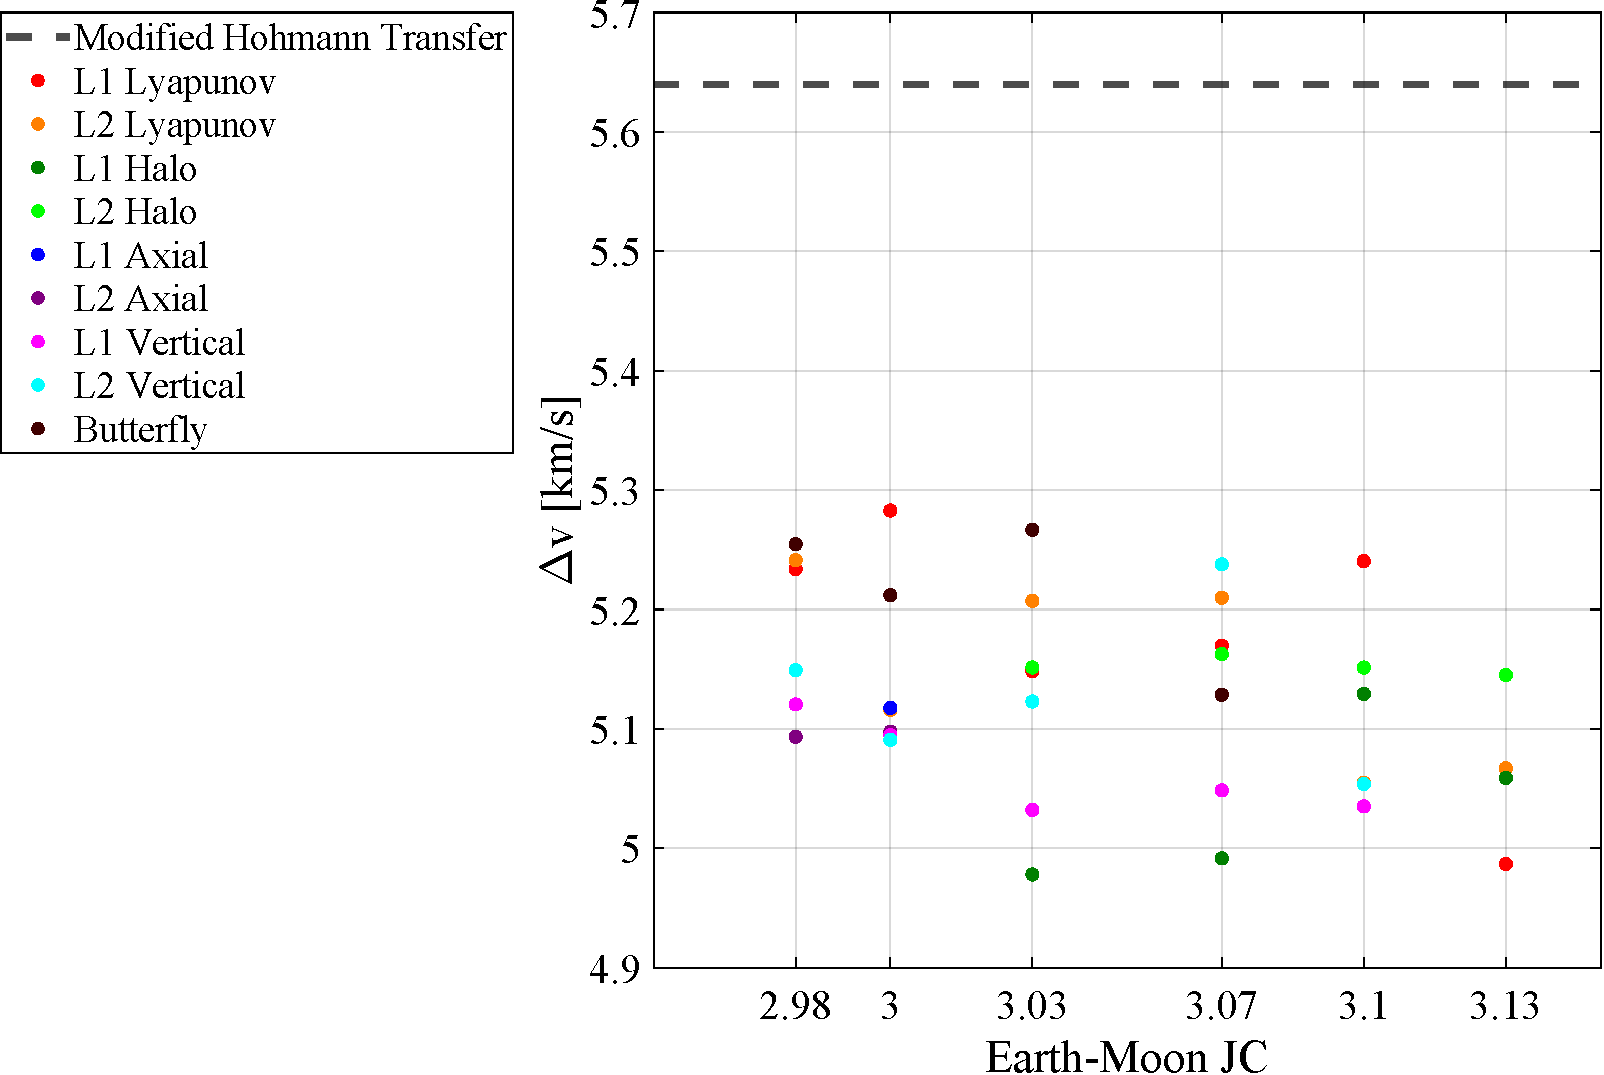
\includegraphics[width=0.9\textwidth]{figures/DeltavComparisonStaged.pdf}
    \caption{Average $\Delta v$ comparison between lowest-cost transfers with staging orbits from various orbits/families.}
    \label{fig:compareDeltavStaged}
\end{figure}

For both categories of transfers, $L_{1}$ orbit families appear to produce lower-$\Delta v$
transfers. It is likely that many of the transfers with invariant manifold arcs originating from
Earth-Moon $L_{1}$ departure families leverage close passes by the Moon to lessen the eventual
energy gap between the planetary systems, resulting in decreased maneuver costs. Again comparing
the two transfer types, in general, the lowest-cost transfers with direct departures outperform the
lowest-cost transfers with staging orbits in terms of maneuver costs. Nevertheless, both types see
cost reduction compared to the baseline modified Hohmann transfer.

When comparing the total transfer TOF between the two categories, the differences are large enough
to be evaluated directly in a single figure. \cref{fig:compareTOF} provides the average lowest-cost
TOF values for both staging orbit transfers and those with direct departures. The staging orbit
transfers all lie in the range of $4.7$-$5.5$ years, while the direct transfer times-of-flight are
significantly lower in comparison: $3.9$-$4.6$ years. It is interesting to note that the energy
levels with higher times-of-flight for the staging orbit transfers are not the same as the higher
TOF options for direct transfers. The spread in TOF between the families at each Jacobi constant
value fluctuates both within each transfer type and overall. For instance, the $3.1$ direct
transfers have a spread of about $0.15$ years while it is $0.6$ at a Jacobi constant of $2.98$, and
the spread is near $0.3$ years for staged orbits at a Jacobi constant of $3.03$ but $0.6$ years for
a $3.07$ Jacobi constant value. The comparison highlights the significant time savings achievable
with direct transfers, while the variability in transfer times across different orbit families
underscores the importance of carefully selecting the optimal departure orbit for minimizing TOF.

\begin{figure}[H]
    \centering
    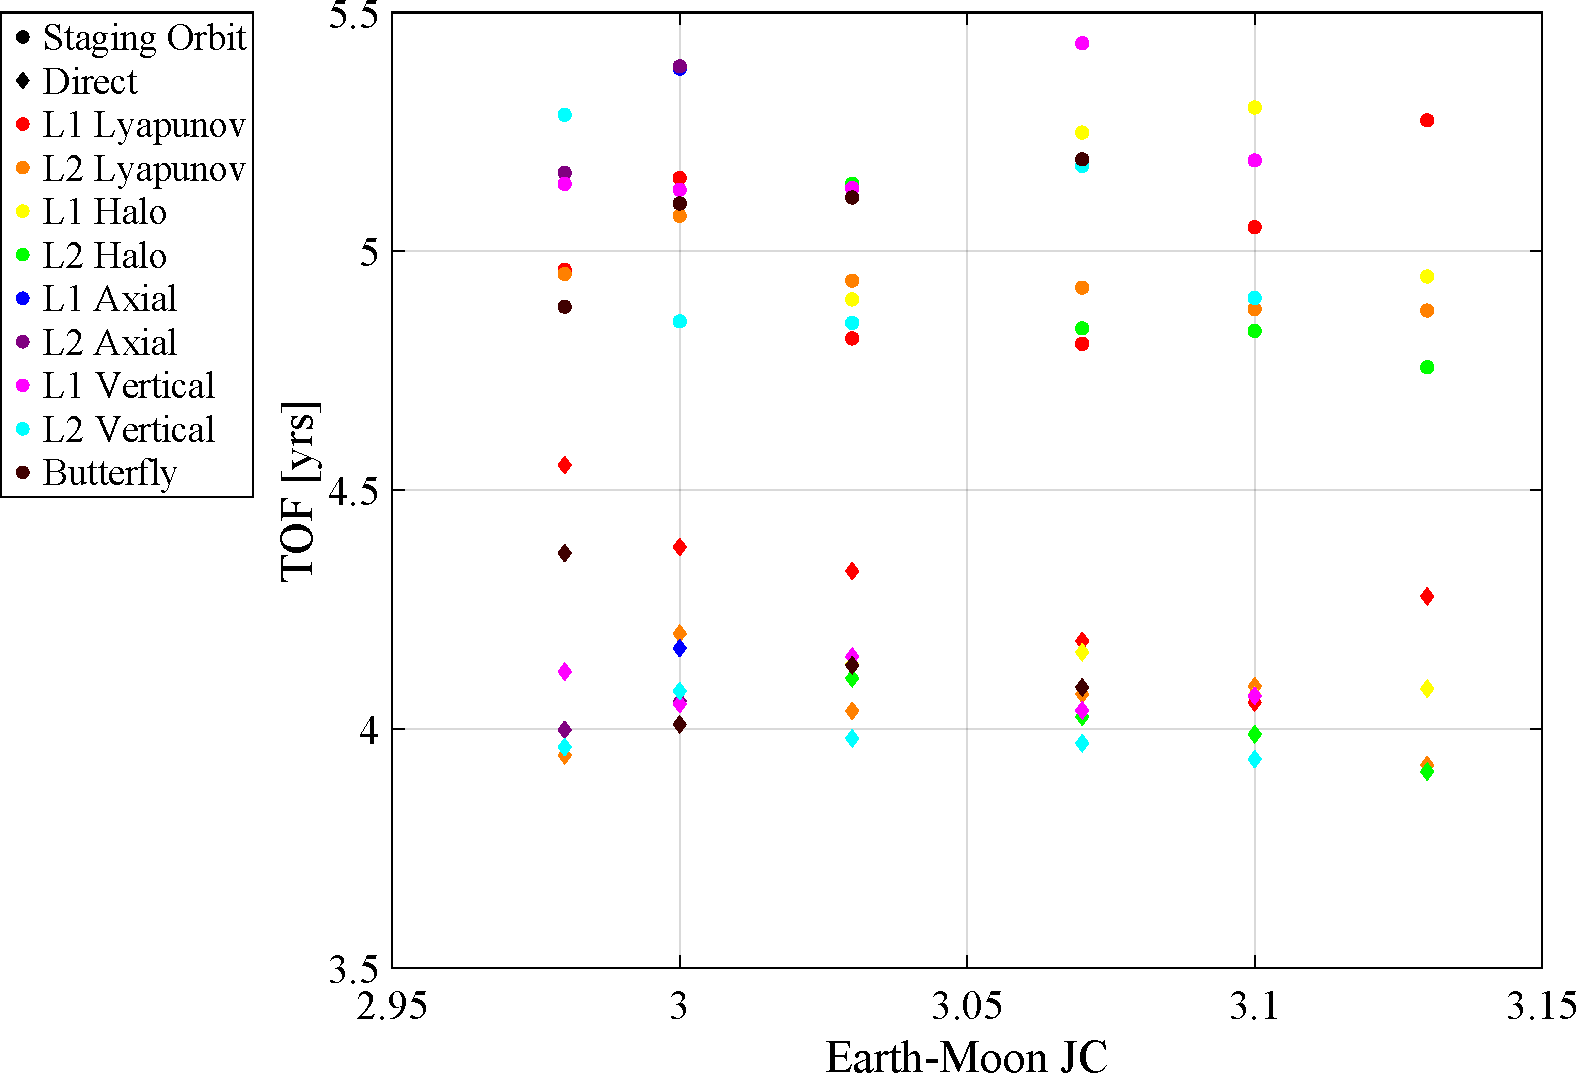
\includegraphics[width=0.9\textwidth]{figures/TOFComparison.pdf}
    \caption{Average TOF comparison between lowest-cost transfers from various orbits/families.}
    \label{fig:compareTOF}
\end{figure}

Like with the total $\Delta v$ costs, the lowest-cost total TOF values fluctuate unpredictably
across each family of orbits. Regardless, for the transfers with staging orbits, the $L_{2}$
Lyapunov and $L_{2}$ halo orbits perform the best overall in TOF, although the results are a little
less clear than when comparing the $\Delta v$ costs. The lowest TOF option investigated is the
$3.13$ $L_{2}$ northern halo orbit, with an average total TOF of $4.76$ years, appearing in
\cref{fig:stagedMinTOFEM}-\cref{fig:stagedMinTOFMMAT}. With the staging orbit transfer type, the
families that perform the worst are the $L_{1}$ vertical and $L_{2}$ axial families. For the direct
transfers, the $L_{2}$ halo and $L_{2}$ vertical orbits have the lowest times-of-flight. The
$L_{2}$ axial orbits also perform well at their limited energy values as with the $\Delta v$. In
the direct category, the $3.13$ $L_{2}$ northern halo orbit again performs the best with an average
total TOF of $3.91$ years, demonstrated in \cref{fig:directMinDvE} and \cref{fig:directMinDvMMAT}.
The ones that have the longest times-of-flight are the $L_{1}$ Lyapunov and halo families. While
$L_{1}$ departure orbits appear to provide lower maneuver costs, \cref{fig:compareTOF} displays
that $L_{2}$ departure orbits tend to have lower times-of-flight, likely because the $L_{2}$
manifold arcs reach the Earth SoI faster and extend slightly farther, decreasing the TOF of the
transfer. Overall, while the $L_{1}$ orbits offer advantages in terms of maneuver cost, the $L_{2}$
orbits are generally more efficient in reducing transfer times.

\begin{figure}[H]
    \centering
    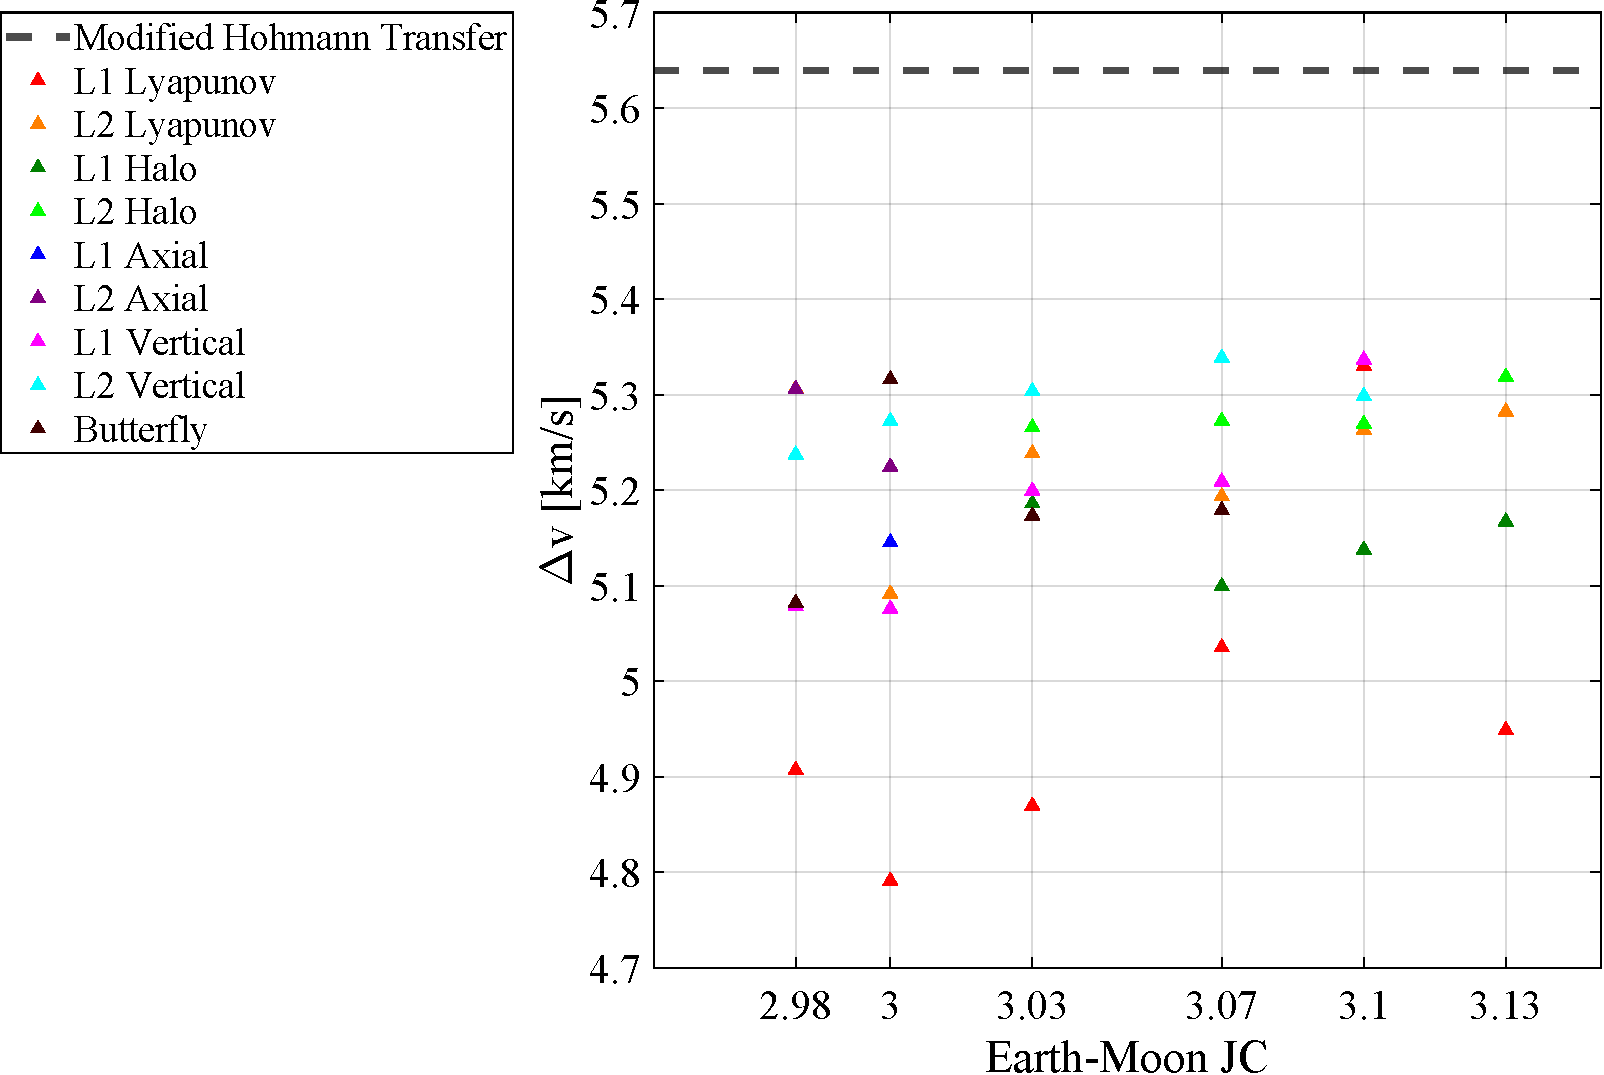
\includegraphics[width=0.9\textwidth]{figures/DeltavComparisonDirect.pdf}
    \caption{Average $\Delta v$ comparison between lowest-cost transfers with direct departures from various orbits/families.}
    \label{fig:compareDeltavDirect}
\end{figure}

Many of the previous examples demonstrate that the transfers with lower total $\Delta v$ tend to
have higher times-of-flight and vice versa. Consequently, to find the departure orbits that provide
decreases in both, the lowest-cost solutions are compared employing $J$, the cost function value.
The results of the comparison appear in \cref{fig:compareJ}. Immediately, it is clear once again
that the transfers with direct departures outperform those with staging orbits, with $J$ values
near $31$ and $36$ respectively. Note that the $J$ values have little physical significance but are
a linear combination of the $\Delta v$ and TOF. The $J$ value spread at each Jacobi constant value
is similar to the spread in TOF in \cref{fig:compareTOF}. Consequently, the direct departure
transfers consistently provide a better balance of maneuver cost and time-of-flight, as indicated
by their lower $J$ values compared to the staging orbit transfers.

\begin{figure}[H]
    \centering
    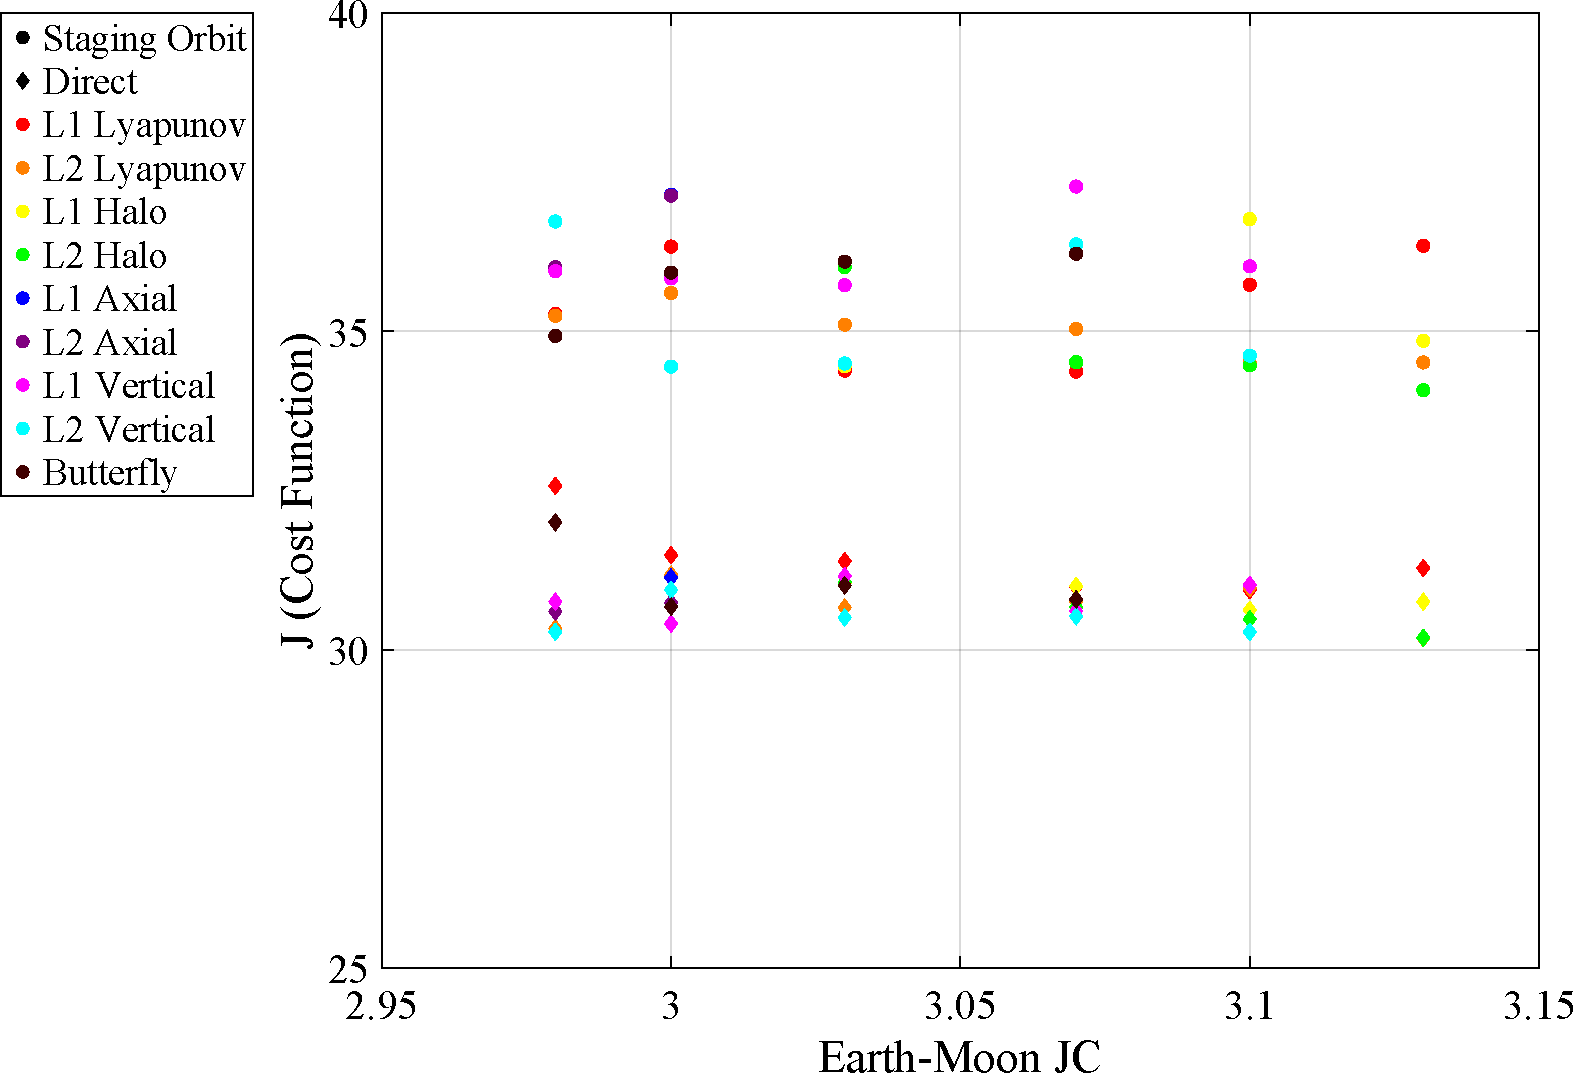
\includegraphics[width=0.9\textwidth]{figures/JComparison.pdf}
    \caption{Average cost function value comparison between lowest-cost transfers from various orbits/families.}
    \label{fig:compareJ}
\end{figure}

In general, comparing the $J$ values between the departure orbits, it is less clear which families
perform the best. For the staging orbits, the $L_{2}$ halo orbits have lower costs at the higher
Jacobi constant values. At the lower Jacobi constants, the better families are different for each
case, although the $L_{2}$ Lyapunov orbits are consistently low throughout. Comparing the direct
transfers, the $L_{2}$ vertical orbit family performs well across the majority of the energy range,
with the $L_{2}$ halos again having low values at higher Jacobi constant orbits. Still within the
direct transfer category, the $L_{1}$ Lyapunov family performs the worst when evaluated with the
cost function. The lowest overall cost departure orbit is the $3.13$ $L_{2}$ Lyapunov orbit direct
departure, with an average cost function value of $30.19$, an average total maneuver cost of
$5.282$ km/s, and an average total TOF of $3.92$ years. The lowest-cost direct transfer from the
departure orbit appears in \cref{fig:bestMMAT} and \cref{fig:bestE} with a total maneuver cost of
$5.293$ km/s and TOF of $3.24$ years. Ultimately, while the comparison of $J$ values reveals
varying performance across different orbit families, the $3.13$ $L_{2}$ Lyapunov orbit direct
departure emerges as the lowest-cost option overall.
\vspace{20mm}

\begin{figure}[H]
    \centering
    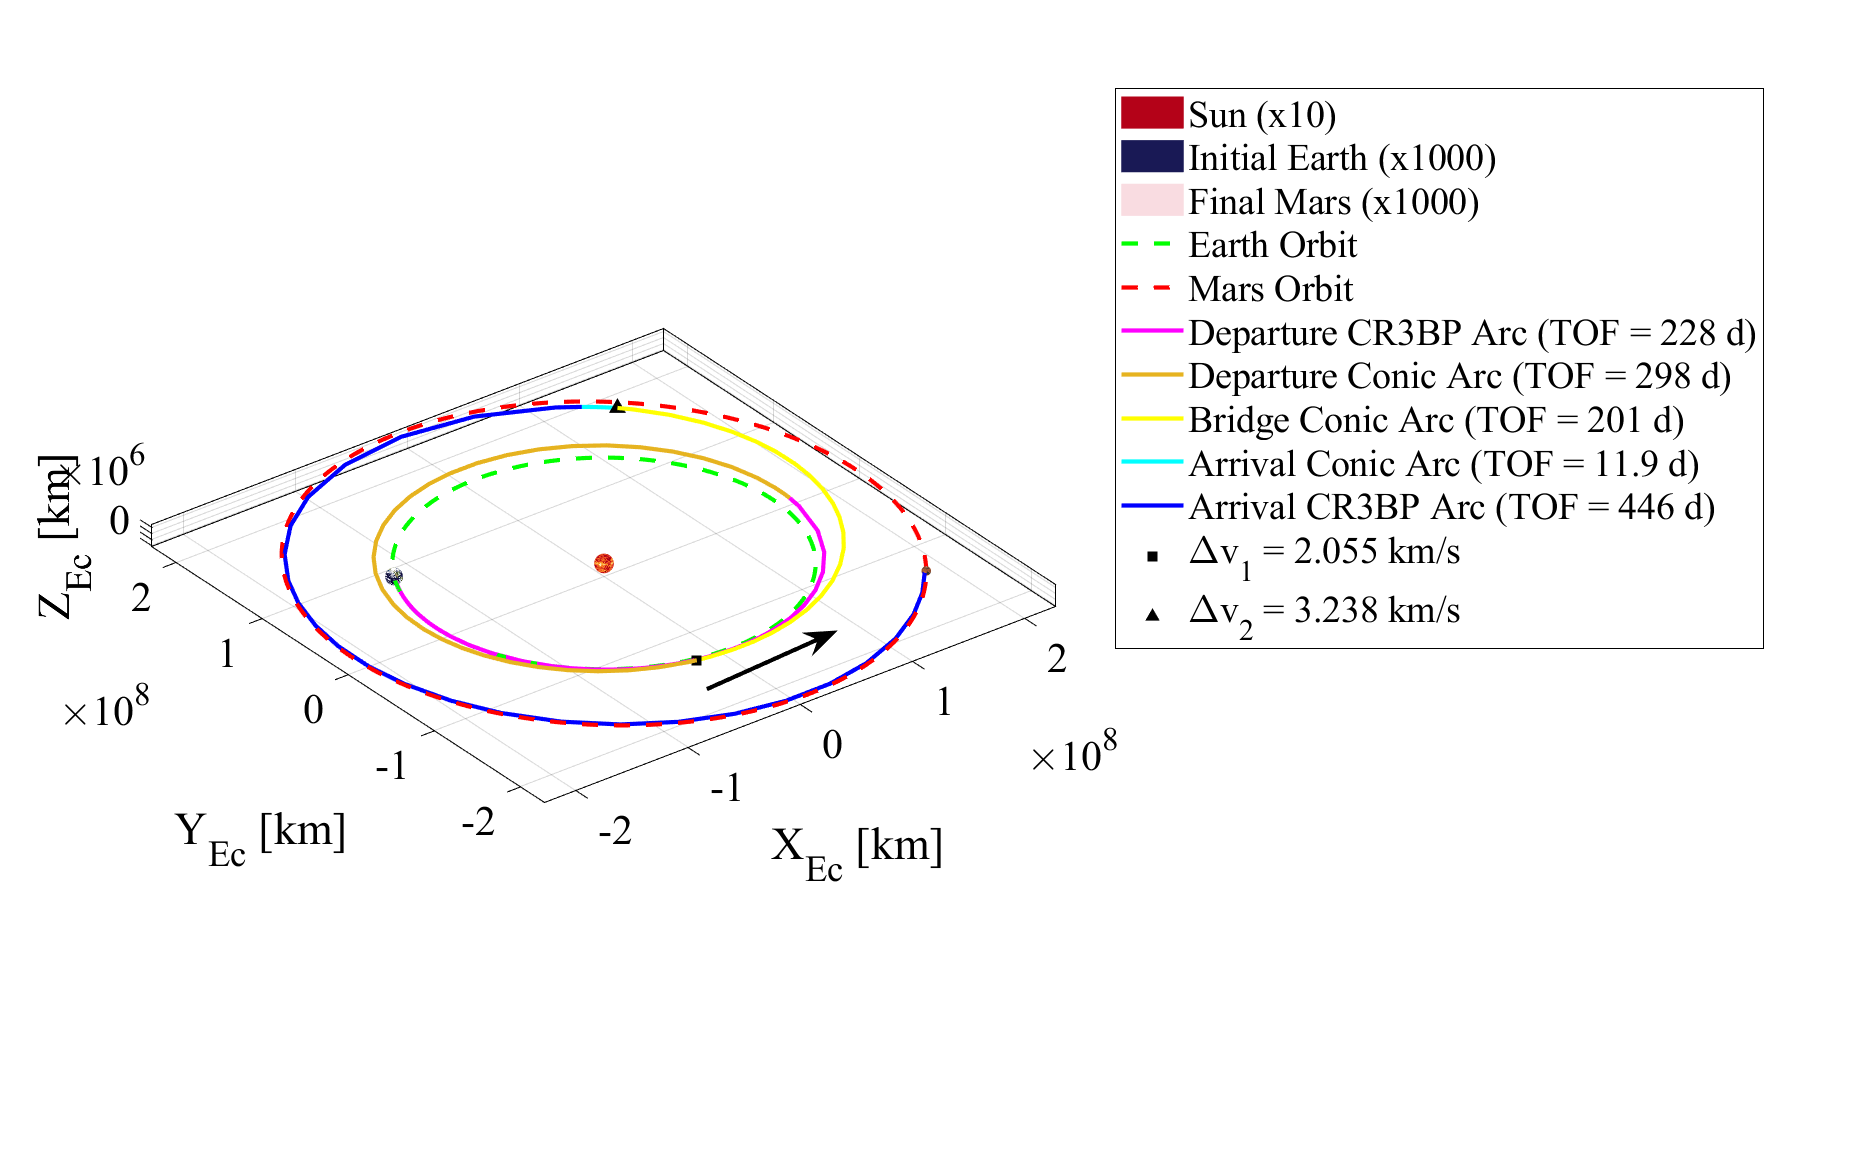
\includegraphics[width=0.9\textwidth]{figures/BestMMAT.pdf}
    \caption{MMAT in the Sun-centered Ecliptic J2000 frame for lowest-cost case.}
    \label{fig:bestMMAT}
\end{figure}

\begin{figure}[H]
    \begin{subfigure}[h]{0.495\linewidth}
        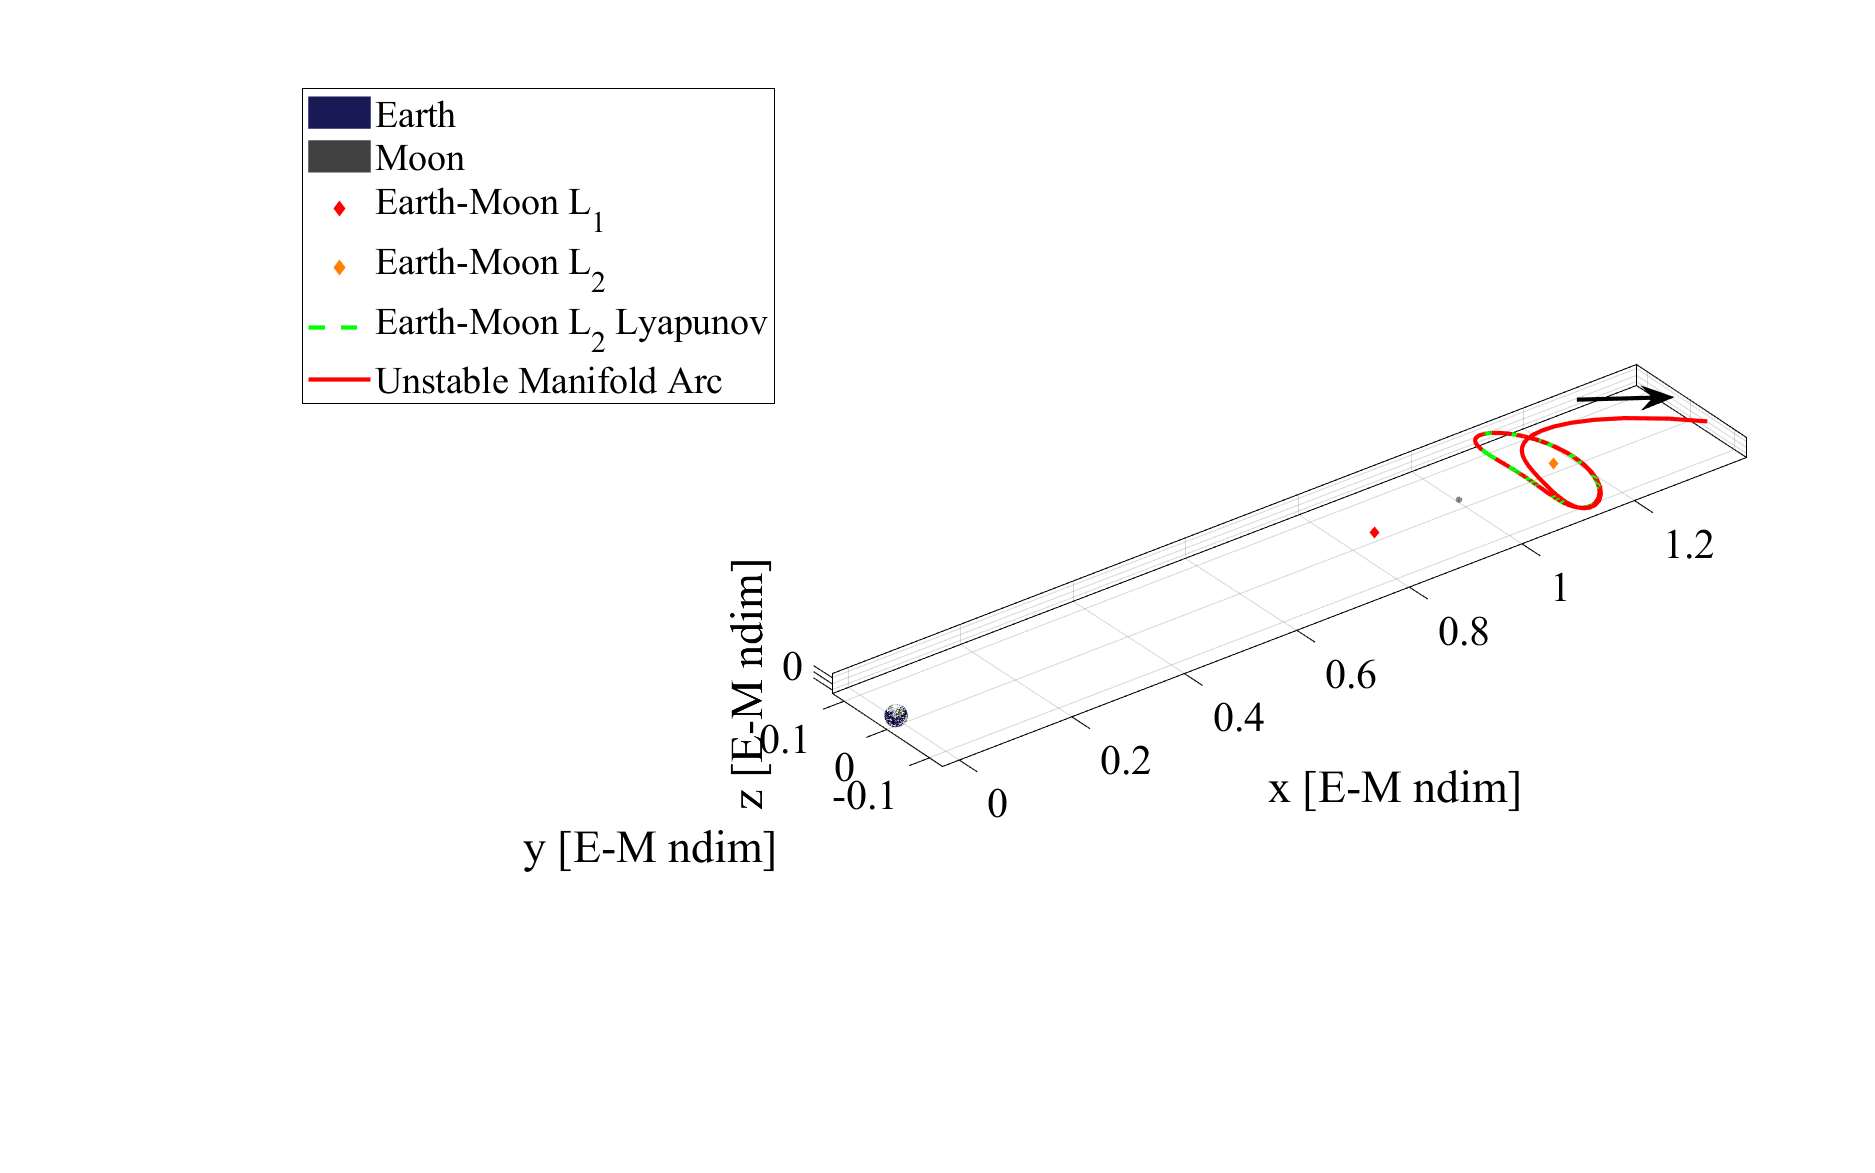
\includegraphics[width=\textwidth]{figures/BestEM.pdf}
        \caption{Earth-Moon barycentric rotating frame.}
    \end{subfigure}
    \hfill
    \begin{subfigure}[h]{0.495\linewidth}
        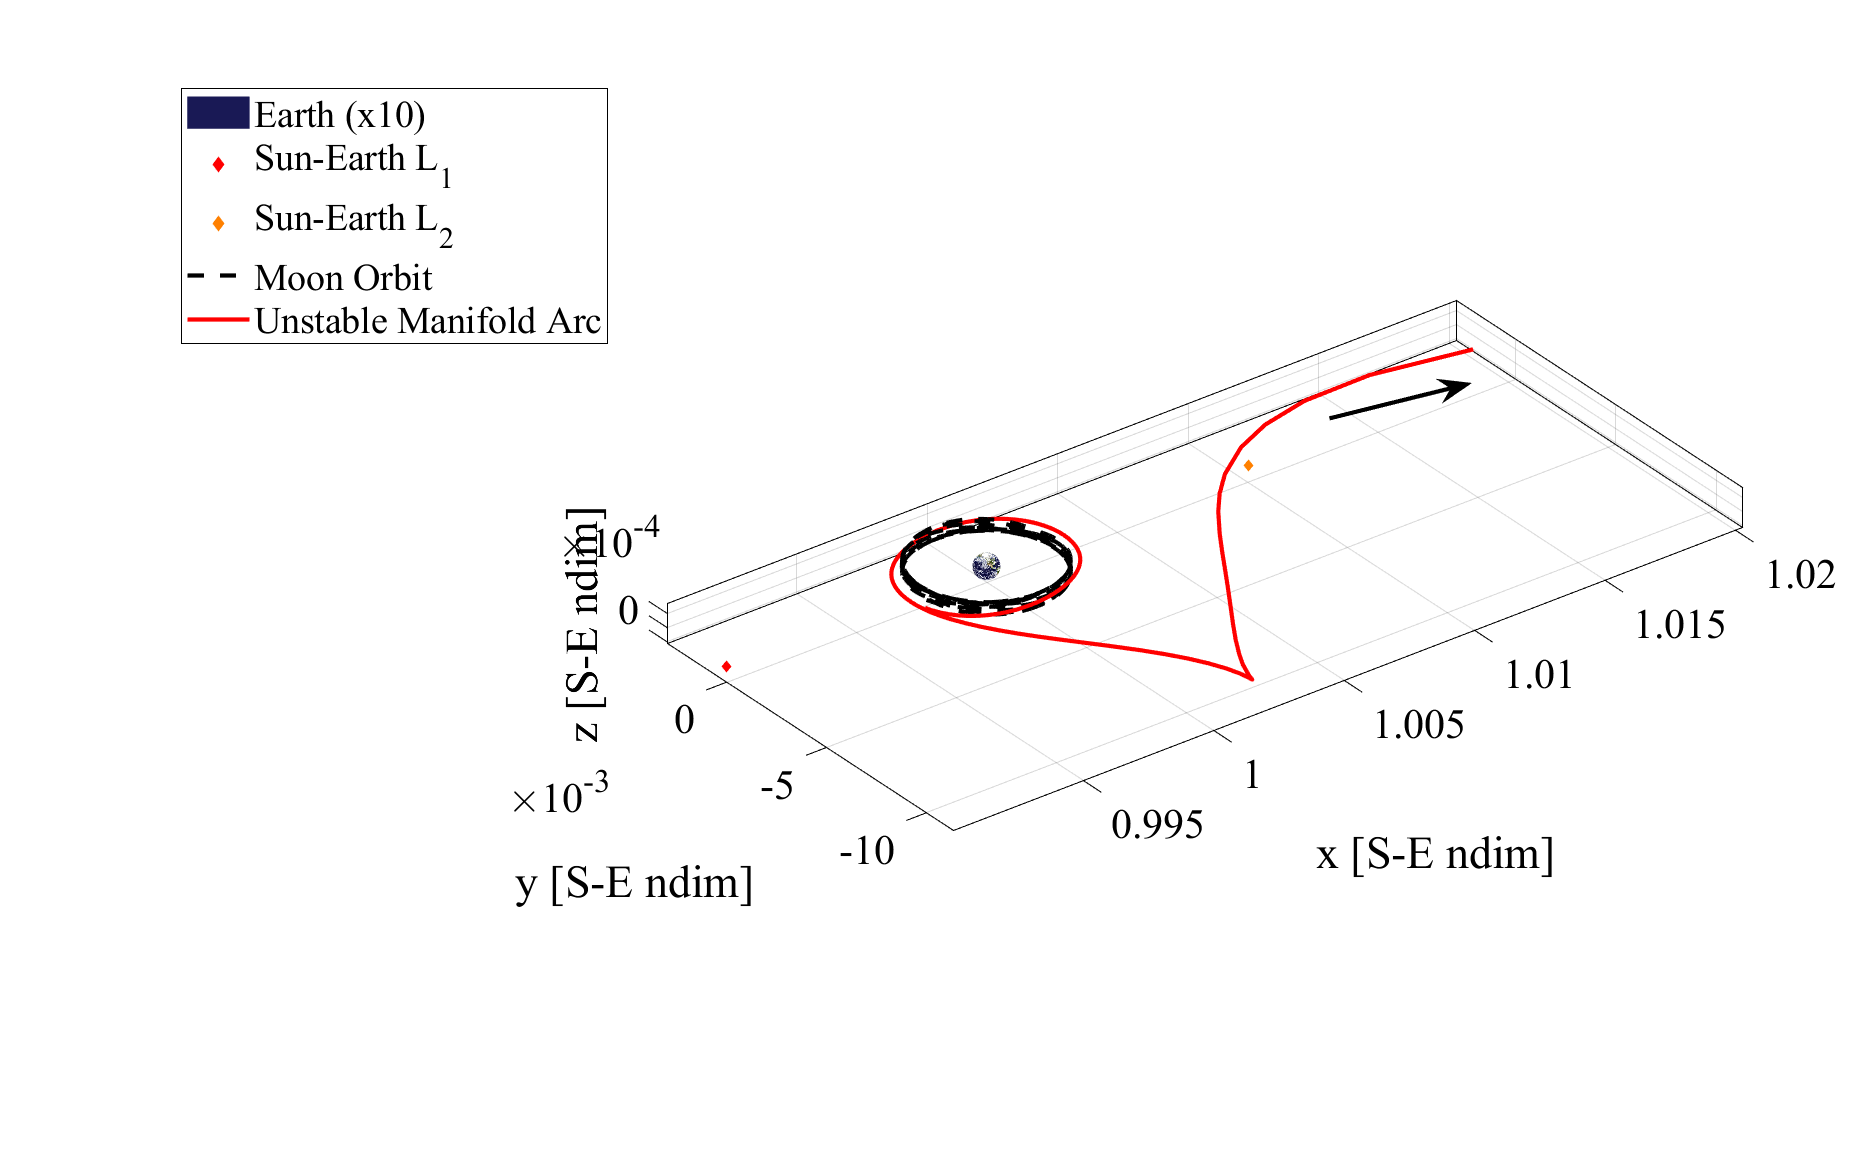
\includegraphics[width=\textwidth]{figures/BestSE.pdf}
        \caption{Sun-Earth barycentric rotating frame.}
    \end{subfigure}
    \caption{$L_{2}$ Lyapunov orbit ($JC=3.13$) departure CR3BP arc for lowest-cost case.}
    \label{fig:bestE}
\end{figure}
